% Options for packages loaded elsewhere
\PassOptionsToPackage{unicode}{hyperref}
\PassOptionsToPackage{hyphens}{url}
%
\documentclass[
]{book}
\usepackage{amsmath,amssymb}
\usepackage{iftex}
\ifPDFTeX
  \usepackage[T1]{fontenc}
  \usepackage[utf8]{inputenc}
  \usepackage{textcomp} % provide euro and other symbols
\else % if luatex or xetex
  \usepackage{unicode-math} % this also loads fontspec
  \defaultfontfeatures{Scale=MatchLowercase}
  \defaultfontfeatures[\rmfamily]{Ligatures=TeX,Scale=1}
\fi
\usepackage{lmodern}
\ifPDFTeX\else
  % xetex/luatex font selection
\fi
% Use upquote if available, for straight quotes in verbatim environments
\IfFileExists{upquote.sty}{\usepackage{upquote}}{}
\IfFileExists{microtype.sty}{% use microtype if available
  \usepackage[]{microtype}
  \UseMicrotypeSet[protrusion]{basicmath} % disable protrusion for tt fonts
}{}
\makeatletter
\@ifundefined{KOMAClassName}{% if non-KOMA class
  \IfFileExists{parskip.sty}{%
    \usepackage{parskip}
  }{% else
    \setlength{\parindent}{0pt}
    \setlength{\parskip}{6pt plus 2pt minus 1pt}}
}{% if KOMA class
  \KOMAoptions{parskip=half}}
\makeatother
\usepackage{xcolor}
\usepackage{color}
\usepackage{fancyvrb}
\newcommand{\VerbBar}{|}
\newcommand{\VERB}{\Verb[commandchars=\\\{\}]}
\DefineVerbatimEnvironment{Highlighting}{Verbatim}{commandchars=\\\{\}}
% Add ',fontsize=\small' for more characters per line
\usepackage{framed}
\definecolor{shadecolor}{RGB}{248,248,248}
\newenvironment{Shaded}{\begin{snugshade}}{\end{snugshade}}
\newcommand{\AlertTok}[1]{\textcolor[rgb]{0.94,0.16,0.16}{#1}}
\newcommand{\AnnotationTok}[1]{\textcolor[rgb]{0.56,0.35,0.01}{\textbf{\textit{#1}}}}
\newcommand{\AttributeTok}[1]{\textcolor[rgb]{0.13,0.29,0.53}{#1}}
\newcommand{\BaseNTok}[1]{\textcolor[rgb]{0.00,0.00,0.81}{#1}}
\newcommand{\BuiltInTok}[1]{#1}
\newcommand{\CharTok}[1]{\textcolor[rgb]{0.31,0.60,0.02}{#1}}
\newcommand{\CommentTok}[1]{\textcolor[rgb]{0.56,0.35,0.01}{\textit{#1}}}
\newcommand{\CommentVarTok}[1]{\textcolor[rgb]{0.56,0.35,0.01}{\textbf{\textit{#1}}}}
\newcommand{\ConstantTok}[1]{\textcolor[rgb]{0.56,0.35,0.01}{#1}}
\newcommand{\ControlFlowTok}[1]{\textcolor[rgb]{0.13,0.29,0.53}{\textbf{#1}}}
\newcommand{\DataTypeTok}[1]{\textcolor[rgb]{0.13,0.29,0.53}{#1}}
\newcommand{\DecValTok}[1]{\textcolor[rgb]{0.00,0.00,0.81}{#1}}
\newcommand{\DocumentationTok}[1]{\textcolor[rgb]{0.56,0.35,0.01}{\textbf{\textit{#1}}}}
\newcommand{\ErrorTok}[1]{\textcolor[rgb]{0.64,0.00,0.00}{\textbf{#1}}}
\newcommand{\ExtensionTok}[1]{#1}
\newcommand{\FloatTok}[1]{\textcolor[rgb]{0.00,0.00,0.81}{#1}}
\newcommand{\FunctionTok}[1]{\textcolor[rgb]{0.13,0.29,0.53}{\textbf{#1}}}
\newcommand{\ImportTok}[1]{#1}
\newcommand{\InformationTok}[1]{\textcolor[rgb]{0.56,0.35,0.01}{\textbf{\textit{#1}}}}
\newcommand{\KeywordTok}[1]{\textcolor[rgb]{0.13,0.29,0.53}{\textbf{#1}}}
\newcommand{\NormalTok}[1]{#1}
\newcommand{\OperatorTok}[1]{\textcolor[rgb]{0.81,0.36,0.00}{\textbf{#1}}}
\newcommand{\OtherTok}[1]{\textcolor[rgb]{0.56,0.35,0.01}{#1}}
\newcommand{\PreprocessorTok}[1]{\textcolor[rgb]{0.56,0.35,0.01}{\textit{#1}}}
\newcommand{\RegionMarkerTok}[1]{#1}
\newcommand{\SpecialCharTok}[1]{\textcolor[rgb]{0.81,0.36,0.00}{\textbf{#1}}}
\newcommand{\SpecialStringTok}[1]{\textcolor[rgb]{0.31,0.60,0.02}{#1}}
\newcommand{\StringTok}[1]{\textcolor[rgb]{0.31,0.60,0.02}{#1}}
\newcommand{\VariableTok}[1]{\textcolor[rgb]{0.00,0.00,0.00}{#1}}
\newcommand{\VerbatimStringTok}[1]{\textcolor[rgb]{0.31,0.60,0.02}{#1}}
\newcommand{\WarningTok}[1]{\textcolor[rgb]{0.56,0.35,0.01}{\textbf{\textit{#1}}}}
\usepackage{longtable,booktabs,array}
\usepackage{calc} % for calculating minipage widths
% Correct order of tables after \paragraph or \subparagraph
\usepackage{etoolbox}
\makeatletter
\patchcmd\longtable{\par}{\if@noskipsec\mbox{}\fi\par}{}{}
\makeatother
% Allow footnotes in longtable head/foot
\IfFileExists{footnotehyper.sty}{\usepackage{footnotehyper}}{\usepackage{footnote}}
\makesavenoteenv{longtable}
\usepackage{graphicx}
\makeatletter
\def\maxwidth{\ifdim\Gin@nat@width>\linewidth\linewidth\else\Gin@nat@width\fi}
\def\maxheight{\ifdim\Gin@nat@height>\textheight\textheight\else\Gin@nat@height\fi}
\makeatother
% Scale images if necessary, so that they will not overflow the page
% margins by default, and it is still possible to overwrite the defaults
% using explicit options in \includegraphics[width, height, ...]{}
\setkeys{Gin}{width=\maxwidth,height=\maxheight,keepaspectratio}
% Set default figure placement to htbp
\makeatletter
\def\fps@figure{htbp}
\makeatother
\setlength{\emergencystretch}{3em} % prevent overfull lines
\providecommand{\tightlist}{%
  \setlength{\itemsep}{0pt}\setlength{\parskip}{0pt}}
\setcounter{secnumdepth}{5}
\usepackage{booktabs}
\usepackage{booktabs}
\usepackage{longtable}
\usepackage{array}
\usepackage{multirow}
\usepackage{wrapfig}
\usepackage{float}
\usepackage{colortbl}
\usepackage{pdflscape}
\usepackage{tabu}
\usepackage{threeparttable}
\usepackage{threeparttablex}
\usepackage[normalem]{ulem}
\usepackage{makecell}
\usepackage{xcolor}
\ifLuaTeX
  \usepackage{selnolig}  % disable illegal ligatures
\fi
\usepackage[]{natbib}
\bibliographystyle{plainnat}
\IfFileExists{bookmark.sty}{\usepackage{bookmark}}{\usepackage{hyperref}}
\IfFileExists{xurl.sty}{\usepackage{xurl}}{} % add URL line breaks if available
\urlstyle{same}
\hypersetup{
  pdftitle={Visualizing NBA},
  pdfauthor={Junqi Fu},
  hidelinks,
  pdfcreator={LaTeX via pandoc}}

\title{Visualizing NBA}
\author{Junqi Fu}
\date{2023-10-21}

\usepackage{amsthm}
\newtheorem{theorem}{Theorem}[chapter]
\newtheorem{lemma}{Lemma}[chapter]
\newtheorem{corollary}{Corollary}[chapter]
\newtheorem{proposition}{Proposition}[chapter]
\newtheorem{conjecture}{Conjecture}[chapter]
\theoremstyle{definition}
\newtheorem{definition}{Definition}[chapter]
\theoremstyle{definition}
\newtheorem{example}{Example}[chapter]
\theoremstyle{definition}
\newtheorem{exercise}{Exercise}[chapter]
\theoremstyle{definition}
\newtheorem{hypothesis}{Hypothesis}[chapter]
\theoremstyle{remark}
\newtheorem*{remark}{Remark}
\newtheorem*{solution}{Solution}
\begin{document}
\maketitle

{
\setcounter{tocdepth}{1}
\tableofcontents
}
\hypertarget{nba-data}{%
\chapter{NBA Data}\label{nba-data}}

The data set contains all the players' performance data from season 1996-97 to season 2022-23.

\hypertarget{data-type}{%
\section{Data Type}\label{data-type}}

Here's a brief explanation of some important variable in the analysis:

\begin{itemize}
\tightlist
\item
  \textbf{player\_height}: player's height in the given season.
\item
  \textbf{player\_weight}: player's weight in the given season.
\item
  \textbf{gp}: total games a player has played in the given season.
\item
  \textbf{pts}: player's average points per game.
\item
  \textbf{reb}: player's average rebound per game.
\item
  \textbf{ast}: player's average assist per game.
\item
  \textbf{net\_rating}: the team's point differential per 100 possessions while a player is on court.
\item
  \textbf{oreb\_pct}: offensive rebound percentage - an estimate of the percentage of available offensive rebounds a player grabbed.
\item
  \textbf{dreb\_pct}: defensive rebound percentage - an estimate of the percentage of available defensive rebounds a player grabbed.
\item
  \textbf{usg\_pct}: usage percentage - an estimate of the percentage of team plays used by a player.
\item
  \textbf{ts\_pct}: true shooting percentage - a measure of shooting efficiency that takes into account field goals, 3-point field goals, and free throws.
\item
  \textbf{ast\_pct}: assist percentage - an estimate of the percentage of teammate field goals a player assisted.
\item
  \textbf{season}: season - the NBA season for which these stats apply.
\end{itemize}

\hypertarget{preliminary-cleaning}{%
\section{Preliminary Cleaning}\label{preliminary-cleaning}}

\hypertarget{initial-missing-data-imputation}{%
\subsection{Initial Missing Data Imputation}\label{initial-missing-data-imputation}}

\begin{Shaded}
\begin{Highlighting}[]
\FunctionTok{sum}\NormalTok{(}\FunctionTok{is.na}\NormalTok{(nba))}
\end{Highlighting}
\end{Shaded}

\begin{verbatim}
## [1] 0
\end{verbatim}

\begin{Shaded}
\begin{Highlighting}[]
\FunctionTok{md.pattern}\NormalTok{(nba)}
\end{Highlighting}
\end{Shaded}

\begin{verbatim}
##  /\     /\
## {  `---'  }
## {  O   O  }
## ==>  V <==  No need for mice. This data set is completely observed.
##  \  \|/  /
##   `-----'
\end{verbatim}

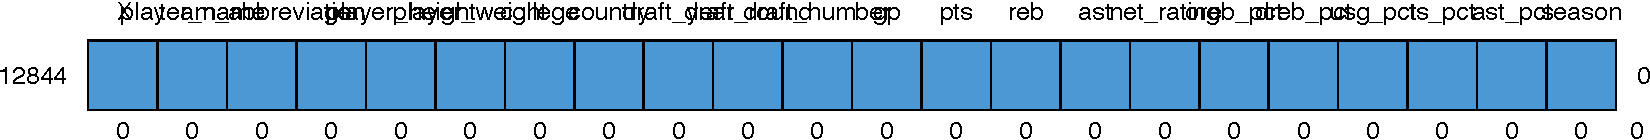
\includegraphics{_main_files/figure-latex/unnamed-chunk-2-1.pdf}

\begin{verbatim}
##       X player_name team_abbreviation age player_height player_weight college
## 12844 1           1                 1   1             1             1       1
##       0           0                 0   0             0             0       0
##       country draft_year draft_round draft_number gp pts reb ast net_rating
## 12844       1          1           1            1  1   1   1   1          1
##             0          0           0            0  0   0   0   0          0
##       oreb_pct dreb_pct usg_pct ts_pct ast_pct season  
## 12844        1        1       1      1       1      1 0
##              0        0       0      0       0      0 0
\end{verbatim}

\begin{Shaded}
\begin{Highlighting}[]
\FunctionTok{md.pattern}\NormalTok{(}\FunctionTok{subset}\NormalTok{(nba,}\AttributeTok{select=}\FunctionTok{c}\NormalTok{(player\_height,player\_weight,gp,pts,reb,ast,net\_rating)))}
\end{Highlighting}
\end{Shaded}

\begin{verbatim}
##  /\     /\
## {  `---'  }
## {  O   O  }
## ==>  V <==  No need for mice. This data set is completely observed.
##  \  \|/  /
##   `-----'
\end{verbatim}

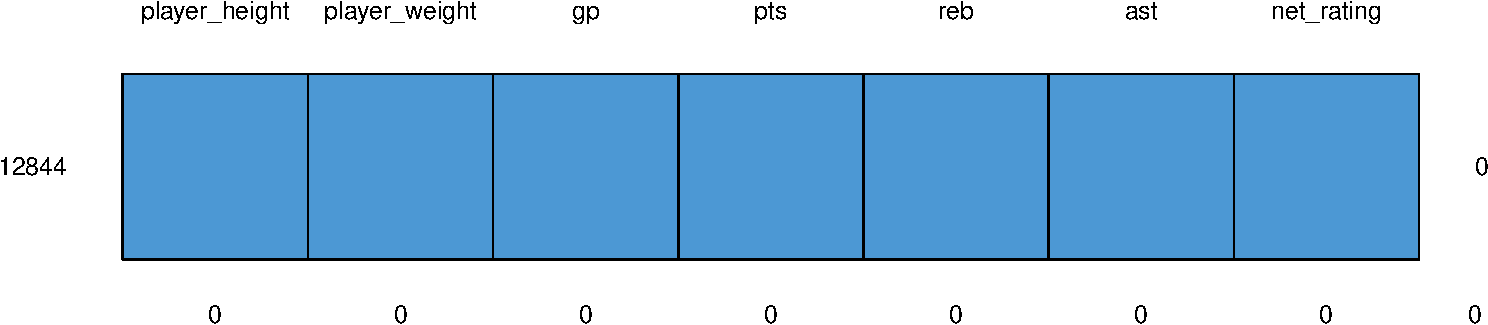
\includegraphics{_main_files/figure-latex/unnamed-chunk-2-2.pdf}

\begin{verbatim}
##       player_height player_weight gp pts reb ast net_rating  
## 12844             1             1  1   1   1   1          1 0
##                   0             0  0   0   0   0          0 0
\end{verbatim}

\begin{Shaded}
\begin{Highlighting}[]
\FunctionTok{aggr}\NormalTok{(}\FunctionTok{subset}\NormalTok{(nba,}\AttributeTok{select=}\FunctionTok{c}\NormalTok{(player\_height,player\_weight,gp,pts,reb,ast,net\_rating)),}\AttributeTok{prop=}\NormalTok{F,}\AttributeTok{numbers=}\ConstantTok{TRUE}\NormalTok{)}
\end{Highlighting}
\end{Shaded}

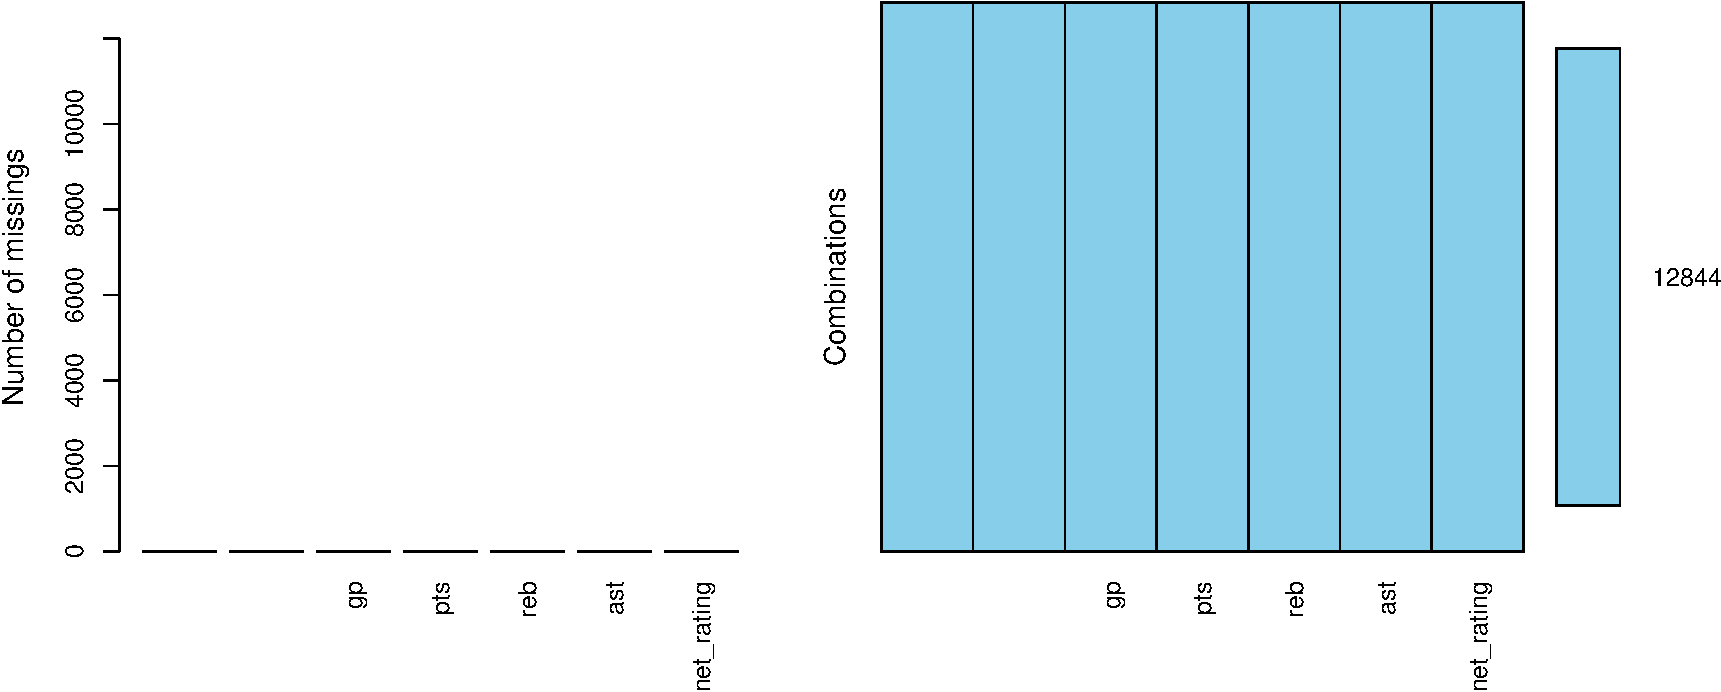
\includegraphics{_main_files/figure-latex/unnamed-chunk-2-3.pdf}

\hypertarget{data-cleaning}{%
\subsection{Data Cleaning}\label{data-cleaning}}

identify outlier exists in the net\_rating, with the 300 as the max and -250 as the min.

\begin{Shaded}
\begin{Highlighting}[]
\FunctionTok{summary}\NormalTok{(nba)}
\end{Highlighting}
\end{Shaded}

\begin{verbatim}
##        X         player_name        team_abbreviation       age       
##  Min.   :    0   Length:12844       Length:12844       Min.   :18.00  
##  1st Qu.: 3211   Class :character   Class :character   1st Qu.:24.00  
##  Median : 6422   Mode  :character   Mode  :character   Median :26.00  
##  Mean   : 6422                                         Mean   :27.05  
##  3rd Qu.: 9632                                         3rd Qu.:30.00  
##  Max.   :12843                                         Max.   :44.00  
##  player_height   player_weight      college            country         
##  Min.   :160.0   Min.   : 60.33   Length:12844       Length:12844      
##  1st Qu.:193.0   1st Qu.: 90.72   Class :character   Class :character  
##  Median :200.7   Median : 99.79   Mode  :character   Mode  :character  
##  Mean   :200.6   Mean   :100.26                                        
##  3rd Qu.:208.3   3rd Qu.:108.86                                        
##  Max.   :231.1   Max.   :163.29                                        
##   draft_year        draft_round        draft_number             gp       
##  Length:12844       Length:12844       Length:12844       Min.   : 1.00  
##  Class :character   Class :character   Class :character   1st Qu.:31.00  
##  Mode  :character   Mode  :character   Mode  :character   Median :57.00  
##                                                           Mean   :51.15  
##                                                           3rd Qu.:73.00  
##                                                           Max.   :85.00  
##       pts              reb              ast           net_rating      
##  Min.   : 0.000   Min.   : 0.000   Min.   : 0.000   Min.   :-250.000  
##  1st Qu.: 3.600   1st Qu.: 1.800   1st Qu.: 0.600   1st Qu.:  -6.400  
##  Median : 6.700   Median : 3.000   Median : 1.200   Median :  -1.300  
##  Mean   : 8.213   Mean   : 3.558   Mean   : 1.825   Mean   :  -2.226  
##  3rd Qu.:11.500   3rd Qu.: 4.700   3rd Qu.: 2.400   3rd Qu.:   3.200  
##  Max.   :36.100   Max.   :16.300   Max.   :11.700   Max.   : 300.000  
##     oreb_pct          dreb_pct         usg_pct           ts_pct      
##  Min.   :0.00000   Min.   :0.0000   Min.   :0.0000   Min.   :0.0000  
##  1st Qu.:0.02100   1st Qu.:0.0960   1st Qu.:0.1490   1st Qu.:0.4820  
##  Median :0.04000   Median :0.1305   Median :0.1810   Median :0.5250  
##  Mean   :0.05407   Mean   :0.1406   Mean   :0.1846   Mean   :0.5131  
##  3rd Qu.:0.08300   3rd Qu.:0.1790   3rd Qu.:0.2170   3rd Qu.:0.5630  
##  Max.   :1.00000   Max.   :1.0000   Max.   :1.0000   Max.   :1.5000  
##     ast_pct          season         
##  Min.   :0.0000   Length:12844      
##  1st Qu.:0.0660   Class :character  
##  Median :0.1030   Mode  :character  
##  Mean   :0.1316                     
##  3rd Qu.:0.1790                     
##  Max.   :1.0000
\end{verbatim}

\begin{Shaded}
\begin{Highlighting}[]
\NormalTok{nba\_clean}\OtherTok{\textless{}{-}}\NormalTok{(}\FunctionTok{which}\NormalTok{(nba}\SpecialCharTok{$}\NormalTok{net\_rating}\SpecialCharTok{\textgreater{}=}\DecValTok{300} \SpecialCharTok{|}\NormalTok{nba}\SpecialCharTok{$}\NormalTok{net\_rating}\SpecialCharTok{\textless{}={-}}\DecValTok{200}\NormalTok{))}
\NormalTok{nba}\OtherTok{\textless{}{-}}\NormalTok{nba[}\SpecialCharTok{{-}}\NormalTok{nba\_clean] }\CommentTok{\#remove the outliers.}
\end{Highlighting}
\end{Shaded}

\hypertarget{preliminary-descriptive-statistics}{%
\section{Preliminary Descriptive Statistics}\label{preliminary-descriptive-statistics}}

\begin{itemize}
\tightlist
\item
  \textbf{age}: the range is between a minimum of 18 years and a maximum of 44 years, with the average age being 26 years old.
\end{itemize}

\begin{Shaded}
\begin{Highlighting}[]
\FunctionTok{summary}\NormalTok{(nba}\SpecialCharTok{$}\NormalTok{age)}
\end{Highlighting}
\end{Shaded}

\begin{verbatim}
##    Min. 1st Qu.  Median    Mean 3rd Qu.    Max. 
##   18.00   24.00   26.00   27.05   30.00   44.00
\end{verbatim}

\begin{itemize}
\tightlist
\item
  \textbf{height}: the range is between a minimum of 160 cm and a maximum of 231.1 cm, with the average height as 200.7 cm.
\end{itemize}

\begin{Shaded}
\begin{Highlighting}[]
\FunctionTok{summary}\NormalTok{(nba}\SpecialCharTok{$}\NormalTok{player\_height)}
\end{Highlighting}
\end{Shaded}

\begin{verbatim}
##    Min. 1st Qu.  Median    Mean 3rd Qu.    Max. 
##   160.0   193.0   200.7   200.6   208.3   231.1
\end{verbatim}

\begin{itemize}
\tightlist
\item
  \textbf{weight}: the range is between a minimum of 60.33 kg and a maximum of 163.29 kg, with the average as 100 kg.
\end{itemize}

\begin{Shaded}
\begin{Highlighting}[]
\FunctionTok{summary}\NormalTok{(nba}\SpecialCharTok{$}\NormalTok{player\_weight)}
\end{Highlighting}
\end{Shaded}

\begin{verbatim}
##    Min. 1st Qu.  Median    Mean 3rd Qu.    Max. 
##   60.33   90.72   99.79  100.26  108.86  163.29
\end{verbatim}

\begin{itemize}
\tightlist
\item
  \textbf{player}: with a highly competitive threshold, only 2551 players have played in the league since 1996.
\end{itemize}

\begin{Shaded}
\begin{Highlighting}[]
\FunctionTok{summary}\NormalTok{(}\FunctionTok{unique}\NormalTok{(nba}\SpecialCharTok{$}\NormalTok{player\_name))}
\end{Highlighting}
\end{Shaded}

\begin{verbatim}
##    Length     Class      Mode 
##      2551 character character
\end{verbatim}

\hypertarget{hypothesis}{%
\chapter{Hypothesis}\label{hypothesis}}

\hypertarget{density-plot-for-height-and-weight}{%
\section{Density Plot for Height and Weight}\label{density-plot-for-height-and-weight}}

\hypertarget{density-plot-for-height-distribution-over-seasons}{%
\subsection{Density Plot for Height Distribution Over Seasons}\label{density-plot-for-height-distribution-over-seasons}}

\begin{Shaded}
\begin{Highlighting}[]
\NormalTok{heightplot }\OtherTok{\textless{}{-}} \FunctionTok{ggplot}\NormalTok{(nba, }\FunctionTok{aes}\NormalTok{(}\AttributeTok{x =}\NormalTok{ player\_height)) }\SpecialCharTok{+}
  \FunctionTok{geom\_density}\NormalTok{(}\FunctionTok{aes}\NormalTok{(}\AttributeTok{fill =}\NormalTok{ season), }\AttributeTok{alpha =} \FloatTok{0.4}\NormalTok{) }\SpecialCharTok{+}
  \FunctionTok{geom\_vline}\NormalTok{(}\FunctionTok{aes}\NormalTok{(}\AttributeTok{xintercept =} \FunctionTok{mean}\NormalTok{(player\_height)), }\AttributeTok{linetype =} \StringTok{"dashed"}\NormalTok{, }\AttributeTok{color =} \StringTok{"red"}\NormalTok{) }\SpecialCharTok{+}
  \FunctionTok{ggtitle}\NormalTok{(}\StringTok{"Density Plot of Player Heights"}\NormalTok{) }\SpecialCharTok{+}
  \FunctionTok{xlab}\NormalTok{(}\StringTok{"Player Height (cm)"}\NormalTok{) }\SpecialCharTok{+}
  \FunctionTok{ylab}\NormalTok{(}\StringTok{"Density"}\NormalTok{) }\SpecialCharTok{+}
  \FunctionTok{theme\_minimal}\NormalTok{()}
\FunctionTok{print}\NormalTok{(heightplot)}
\end{Highlighting}
\end{Shaded}

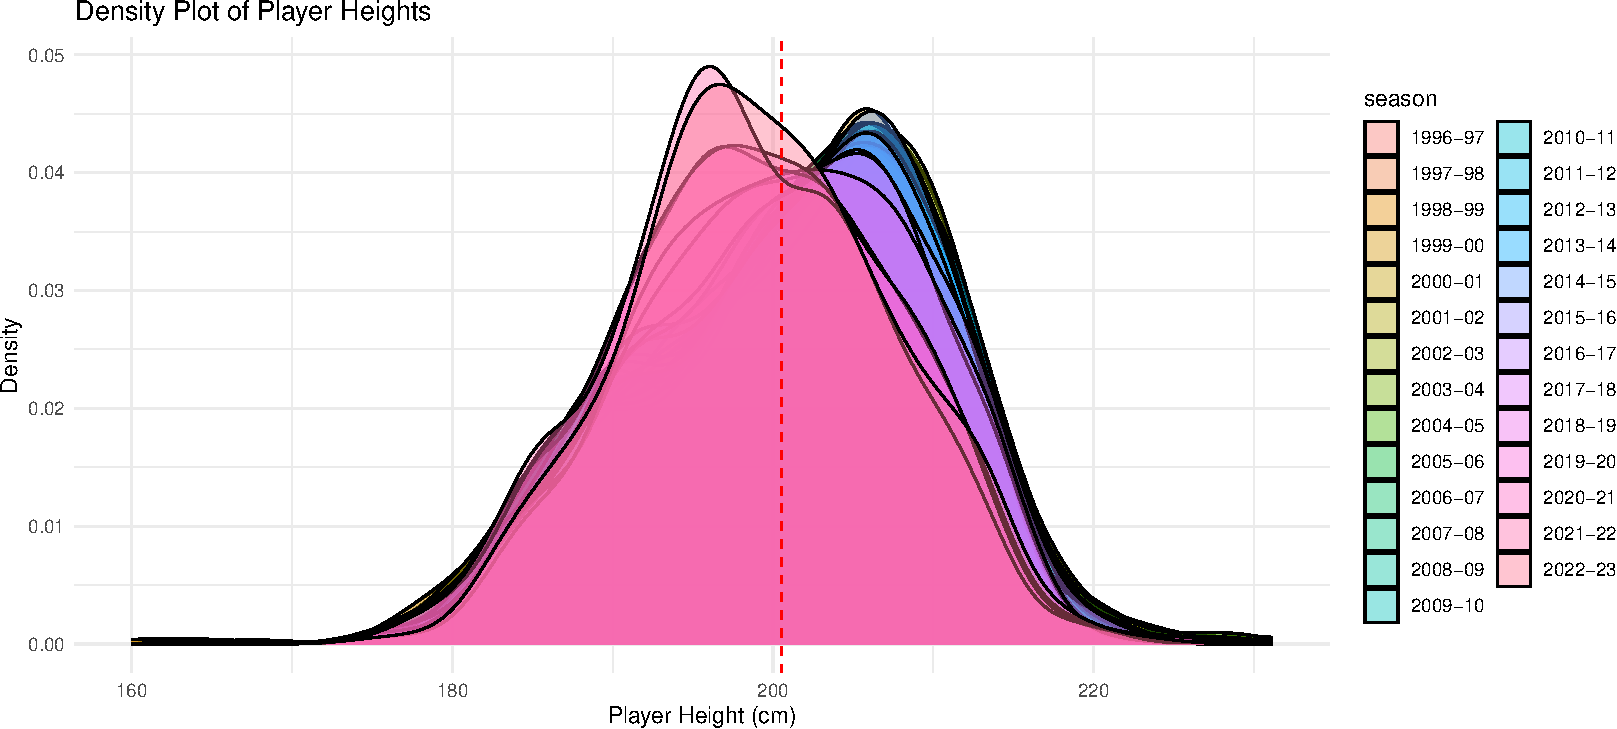
\includegraphics{_main_files/figure-latex/unnamed-chunk-9-1.pdf}

\hypertarget{summary}{%
\subsubsection{Summary}\label{summary}}

\begin{itemize}
\tightlist
\item
  A more noticeable shift in the mean height of players over seasons. The mean height has decreased steadily.
\item
  A narrower range of heights among players in the recent NBA compared to the past.
\item
  There's a noticeable peak around the 200-210 cm range, suggesting that a significant number of players fall within this height bracket.
\end{itemize}

\hypertarget{density-plot-for-weight-distribution-over-seasons}{%
\subsection{Density Plot for Weight Distribution Over Seasons}\label{density-plot-for-weight-distribution-over-seasons}}

\begin{Shaded}
\begin{Highlighting}[]
\NormalTok{weightplot }\OtherTok{\textless{}{-}} \FunctionTok{ggplot}\NormalTok{(nba, }\FunctionTok{aes}\NormalTok{(}\AttributeTok{x =}\NormalTok{ player\_weight)) }\SpecialCharTok{+}
  \FunctionTok{geom\_density}\NormalTok{(}\FunctionTok{aes}\NormalTok{(}\AttributeTok{fill =}\NormalTok{ season), }\AttributeTok{alpha =} \FloatTok{0.4}\NormalTok{) }\SpecialCharTok{+}
  \FunctionTok{geom\_vline}\NormalTok{(}\FunctionTok{aes}\NormalTok{(}\AttributeTok{xintercept =} \FunctionTok{mean}\NormalTok{(player\_weight)), }\AttributeTok{linetype =} \StringTok{"dashed"}\NormalTok{, }\AttributeTok{color =} \StringTok{"red"}\NormalTok{) }\SpecialCharTok{+}
  \FunctionTok{ggtitle}\NormalTok{(}\StringTok{"Density Plot of Player Weights"}\NormalTok{) }\SpecialCharTok{+}
  \FunctionTok{xlab}\NormalTok{(}\StringTok{"Player Weight (kg)"}\NormalTok{) }\SpecialCharTok{+}
  \FunctionTok{ylab}\NormalTok{(}\StringTok{"Density"}\NormalTok{) }\SpecialCharTok{+}
  \FunctionTok{theme\_minimal}\NormalTok{()}
\FunctionTok{print}\NormalTok{(weightplot)}
\end{Highlighting}
\end{Shaded}

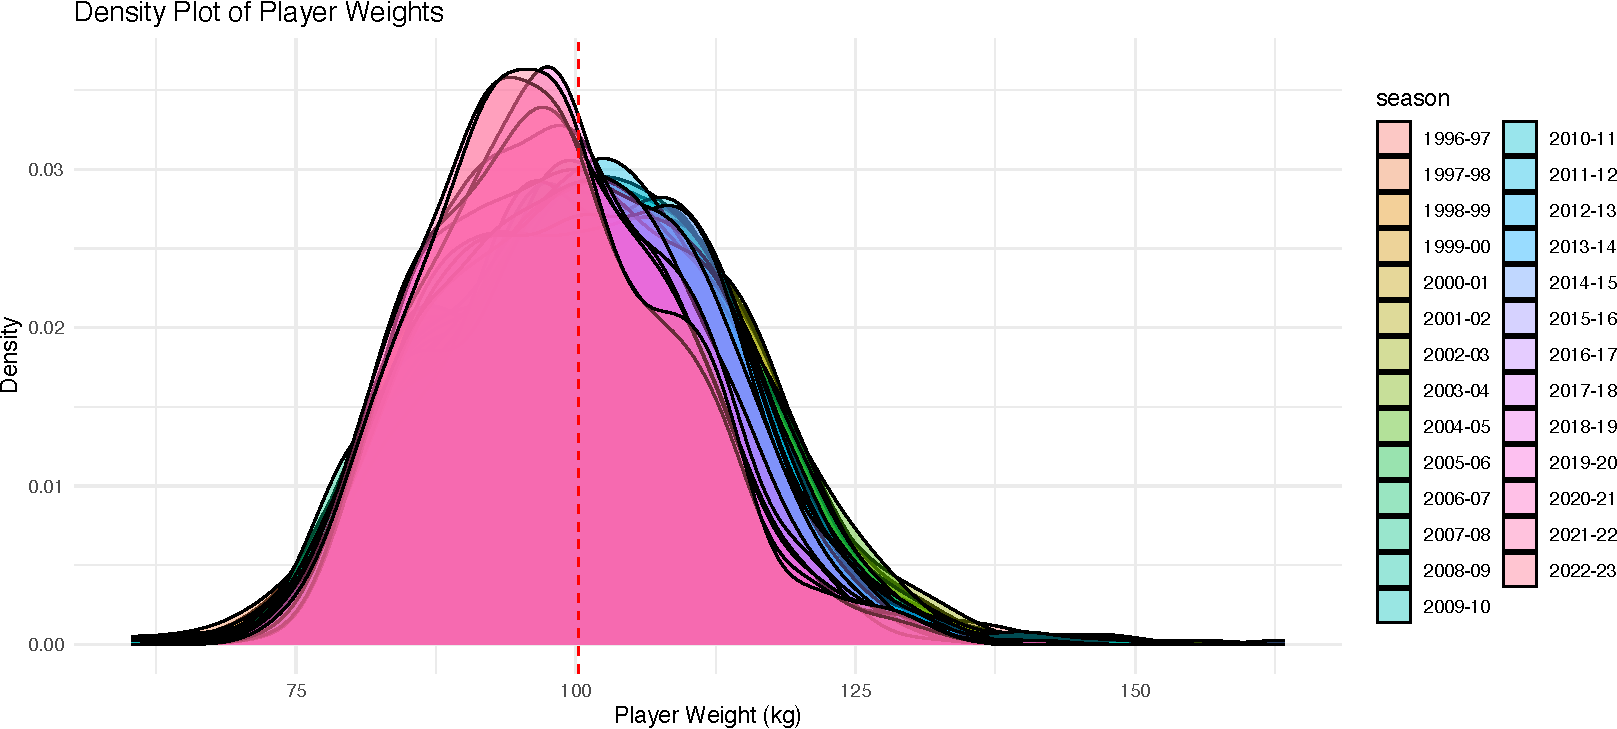
\includegraphics{_main_files/figure-latex/unnamed-chunk-10-1.pdf}

\hypertarget{summary-1}{%
\subsubsection{Summary}\label{summary-1}}

\begin{itemize}
\tightlist
\item
  The mean weight seems to have shifted towards the left, suggesting that players have, on average, become lighter over the years.
\item
  The distributions for the recent seasons appear narrower, indicating less variability in player weights now than in earlier seasons.
\end{itemize}

\hypertarget{in-summary-over-the-years-nba-players-have-on-average-become-shorter-and-lighter-with-a-narrower-range-of-both-weights-and-heights-represented-in-recent-seasons.}{%
\subsection{In summary, over the years, NBA players have, on average, become shorter and lighter, with a narrower range of both weights and heights represented in recent seasons.}\label{in-summary-over-the-years-nba-players-have-on-average-become-shorter-and-lighter-with-a-narrower-range-of-both-weights-and-heights-represented-in-recent-seasons.}}

\hypertarget{inference-hypothesis-based-on-the-density-plot-and-initial-summary}{%
\section{Inference \& Hypothesis Based On The Density Plot and Initial Summary}\label{inference-hypothesis-based-on-the-density-plot-and-initial-summary}}

\begin{itemize}
\tightlist
\item
  \textbf{H1} Versatility \& Position-less Basketball: the narrower range of heights and weights indicates that there might be an increasing trend of ``position-less'' basketball, specifically players are no longer strictly confined to traditional roles based on their physical attributes.
\item
  \textbf{H2} Evolution in Playing Style: the traditional center-focused style of play cannot adapt to the pace of the modern NBA.
\item
  \textbf{H3} Defensive Switching: With players might having a wider range of skills irrespective of their height or weight, teams can employ more switching on defense. Players are more equipped to defend multiple positions, making it harder for offenses to exploit mismatches.
\end{itemize}

\hypertarget{correlation-analysis}{%
\section{Correlation analysis}\label{correlation-analysis}}

\hypertarget{correlation-analysis-between-heightweight-and-other-data}{%
\subsection{Correlation analysis between height/weight and other data}\label{correlation-analysis-between-heightweight-and-other-data}}

\begin{Shaded}
\begin{Highlighting}[]
\FunctionTok{ggplot}\NormalTok{(}\AttributeTok{data =}\NormalTok{ melted\_cormat, }\FunctionTok{aes}\NormalTok{(}\AttributeTok{x=}\NormalTok{Var1, }\AttributeTok{y=}\NormalTok{Var2)) }\SpecialCharTok{+}
  \FunctionTok{geom\_tile}\NormalTok{(}\FunctionTok{aes}\NormalTok{(}\AttributeTok{fill=}\NormalTok{value), }\AttributeTok{color=}\StringTok{\textquotesingle{}white\textquotesingle{}}\NormalTok{) }\SpecialCharTok{+}
  \FunctionTok{scale\_fill\_gradient2}\NormalTok{(}\AttributeTok{low=}\StringTok{\textquotesingle{}blue\textquotesingle{}}\NormalTok{, }\AttributeTok{high=}\StringTok{\textquotesingle{}red\textquotesingle{}}\NormalTok{, }\AttributeTok{mid=}\StringTok{\textquotesingle{}white\textquotesingle{}}\NormalTok{, }\AttributeTok{midpoint=}\DecValTok{0}\NormalTok{, }\AttributeTok{limit=}\FunctionTok{c}\NormalTok{(}\SpecialCharTok{{-}}\DecValTok{1}\NormalTok{,}\DecValTok{1}\NormalTok{), }\AttributeTok{space=}\StringTok{\textquotesingle{}Lab\textquotesingle{}}\NormalTok{, }\AttributeTok{name=}\StringTok{\textquotesingle{}Correlation\textquotesingle{}}\NormalTok{) }\SpecialCharTok{+}
  \FunctionTok{theme\_minimal}\NormalTok{() }\SpecialCharTok{+}
  \FunctionTok{theme}\NormalTok{(}\AttributeTok{axis.text.x=}\FunctionTok{element\_text}\NormalTok{(}\AttributeTok{angle=}\DecValTok{45}\NormalTok{, }\AttributeTok{vjust=}\DecValTok{1}\NormalTok{, }\AttributeTok{size=}\DecValTok{12}\NormalTok{, }\AttributeTok{hjust=}\DecValTok{1}\NormalTok{),}
        \AttributeTok{axis.text.y=}\FunctionTok{element\_text}\NormalTok{(}\AttributeTok{size=}\DecValTok{12}\NormalTok{)) }\SpecialCharTok{+}
  \FunctionTok{coord\_fixed}\NormalTok{()}
\end{Highlighting}
\end{Shaded}

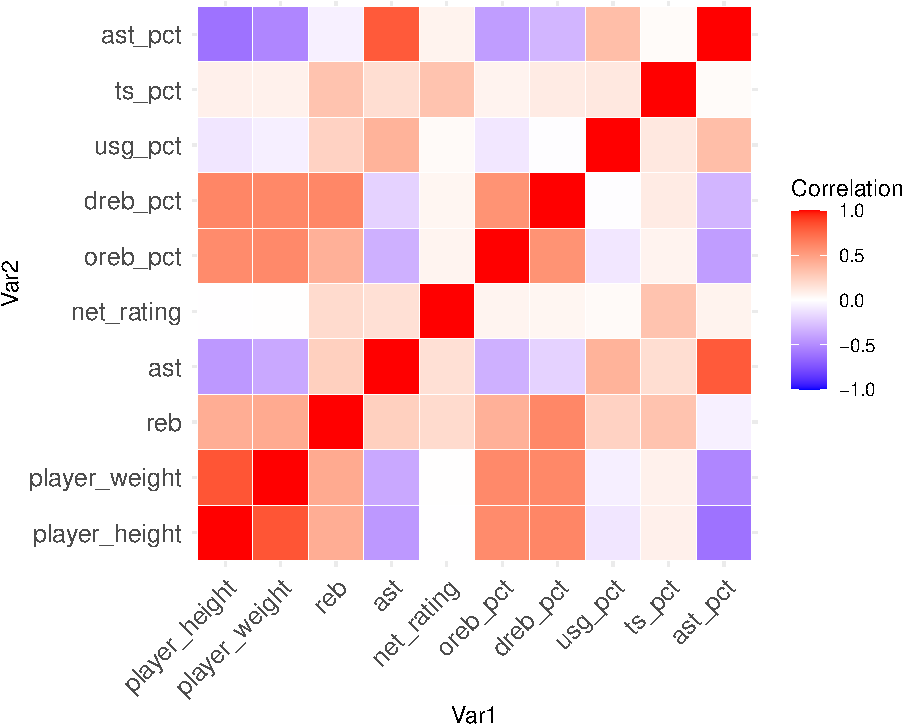
\includegraphics{_main_files/figure-latex/unnamed-chunk-12-1.pdf}

\hypertarget{correlational-matrix.}{%
\subsubsection{Correlational Matrix.}\label{correlational-matrix.}}

\begin{Shaded}
\begin{Highlighting}[]
\FunctionTok{grid.arrange}\NormalTok{(height\_reb}\SpecialCharTok{+}\FunctionTok{geom\_smooth}\NormalTok{(), height\_ast}\SpecialCharTok{+}\FunctionTok{geom\_smooth}\NormalTok{(), weight\_reb}\SpecialCharTok{+}\FunctionTok{geom\_smooth}\NormalTok{(),weight\_ast}\SpecialCharTok{+}\FunctionTok{geom\_smooth}\NormalTok{() , }\AttributeTok{ncol =} \DecValTok{2}\NormalTok{)}
\end{Highlighting}
\end{Shaded}

\begin{verbatim}
## `geom_smooth()` using method = 'gam' and formula = 'y ~ s(x, bs = "cs")'
## `geom_smooth()` using method = 'gam' and formula = 'y ~ s(x, bs = "cs")'
## `geom_smooth()` using method = 'gam' and formula = 'y ~ s(x, bs = "cs")'
## `geom_smooth()` using method = 'gam' and formula = 'y ~ s(x, bs = "cs")'
\end{verbatim}

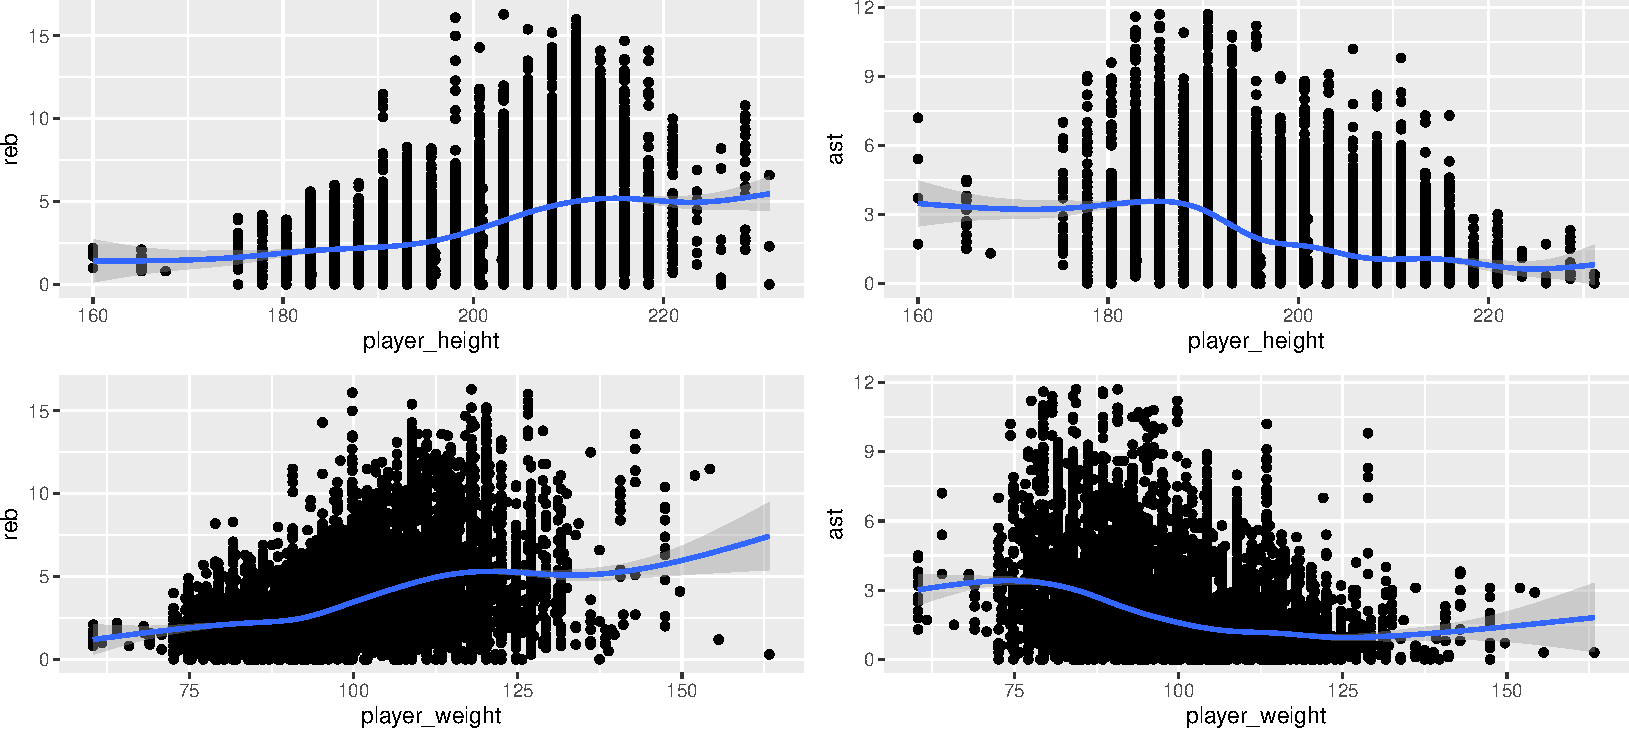
\includegraphics{_main_files/figure-latex/unnamed-chunk-14-1.pdf}

\hypertarget{boxplot}{%
\subsection{Boxplot}\label{boxplot}}

\begin{Shaded}
\begin{Highlighting}[]
\NormalTok{heightdatapart }\OtherTok{\textless{}{-}} \FunctionTok{data.frame}\NormalTok{(}\AttributeTok{player\_height =}\NormalTok{ nba}\SpecialCharTok{$}\NormalTok{player\_height, }\AttributeTok{net\_rating =}\NormalTok{ nba}\SpecialCharTok{$}\NormalTok{net\_rating)}

\NormalTok{heightdatapart }\OtherTok{\textless{}{-}}\NormalTok{ heightdatapart[(heightdatapart}\SpecialCharTok{$}\NormalTok{net\_rating }\SpecialCharTok{\textgreater{}=} \SpecialCharTok{{-}}\DecValTok{50} \SpecialCharTok{\&}\NormalTok{ heightdatapart}\SpecialCharTok{$}\NormalTok{net\_rating }\SpecialCharTok{\textless{}=} \DecValTok{50}\NormalTok{), ]}

\NormalTok{heightdatapart}\SpecialCharTok{$}\NormalTok{group }\OtherTok{\textless{}{-}} \FunctionTok{cut}\NormalTok{(heightdatapart}\SpecialCharTok{$}\NormalTok{player\_height, }\AttributeTok{breaks =} \DecValTok{7}\NormalTok{)}

\NormalTok{ph }\OtherTok{\textless{}{-}} \FunctionTok{ggplot}\NormalTok{(}\AttributeTok{data =}\NormalTok{ heightdatapart, }\FunctionTok{aes}\NormalTok{(}\AttributeTok{x =}\NormalTok{ group, }\AttributeTok{y =}\NormalTok{ net\_rating, }\AttributeTok{fill =}\NormalTok{ group)) }\SpecialCharTok{+}
  \FunctionTok{geom\_boxplot}\NormalTok{() }\SpecialCharTok{+}
  \FunctionTok{ggtitle}\NormalTok{(}\StringTok{"Net Rating by Player Height"}\NormalTok{) }\SpecialCharTok{+}
  \FunctionTok{theme\_minimal}\NormalTok{()}
\FunctionTok{print}\NormalTok{(ph)}
\end{Highlighting}
\end{Shaded}

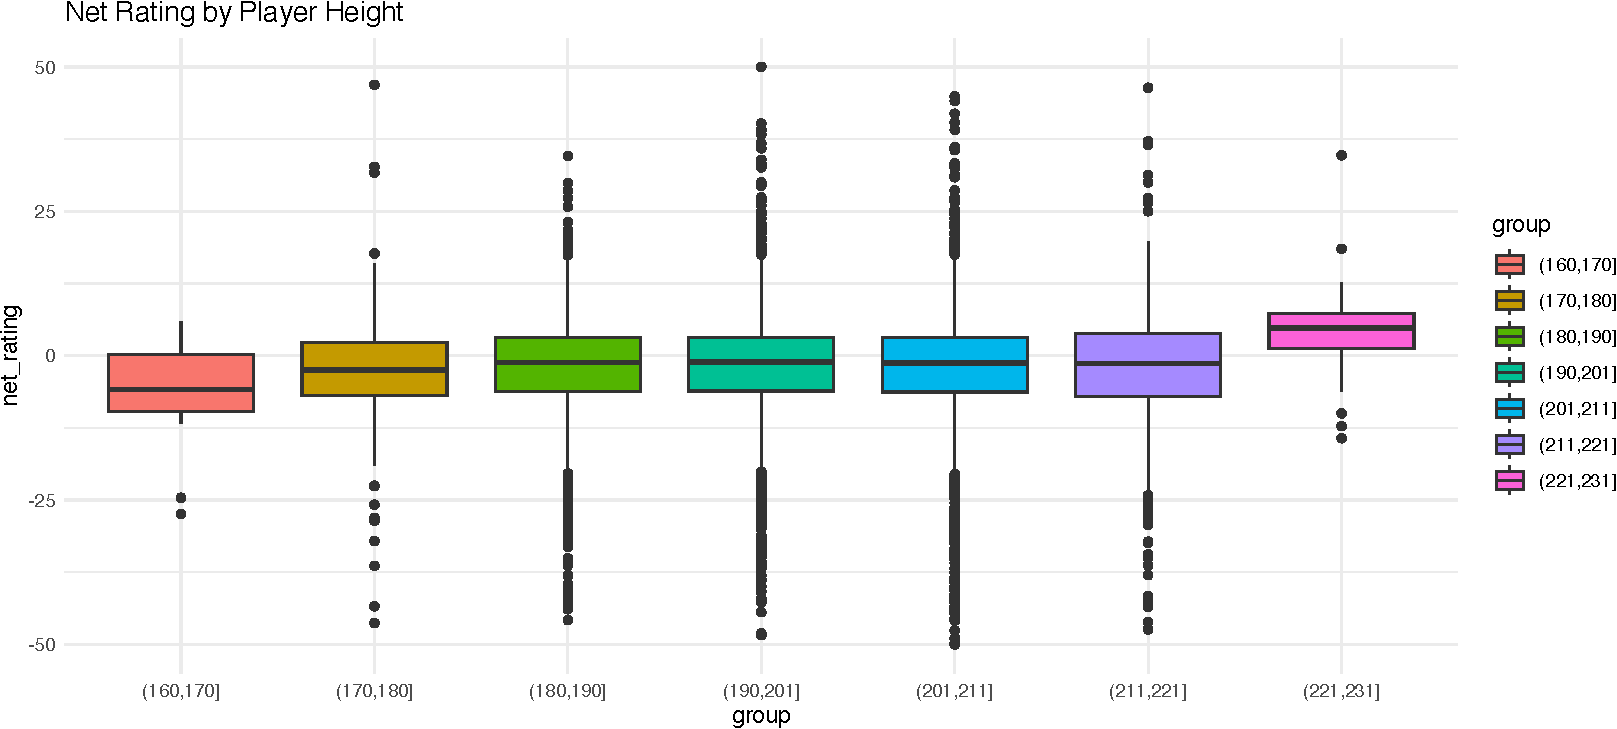
\includegraphics{_main_files/figure-latex/unnamed-chunk-15-1.pdf}

\begin{Shaded}
\begin{Highlighting}[]
\NormalTok{weightdatapart }\OtherTok{\textless{}{-}} \FunctionTok{data.frame}\NormalTok{(}\AttributeTok{player\_weight =}\NormalTok{ nba}\SpecialCharTok{$}\NormalTok{player\_weight, }\AttributeTok{net\_rating =}\NormalTok{ nba}\SpecialCharTok{$}\NormalTok{net\_rating)}

\NormalTok{weightdatapart }\OtherTok{\textless{}{-}}\NormalTok{ weightdatapart[(weightdatapart}\SpecialCharTok{$}\NormalTok{net\_rating }\SpecialCharTok{\textgreater{}=} \SpecialCharTok{{-}}\DecValTok{50} \SpecialCharTok{\&}\NormalTok{ weightdatapart}\SpecialCharTok{$}\NormalTok{net\_rating }\SpecialCharTok{\textless{}=} \DecValTok{50}\NormalTok{), ]}

\NormalTok{weightdatapart}\SpecialCharTok{$}\NormalTok{group }\OtherTok{\textless{}{-}} \FunctionTok{cut}\NormalTok{(weightdatapart}\SpecialCharTok{$}\NormalTok{player\_weight, }\AttributeTok{breaks =} \DecValTok{7}\NormalTok{)}

\NormalTok{pw }\OtherTok{\textless{}{-}} \FunctionTok{ggplot}\NormalTok{(}\AttributeTok{data =}\NormalTok{ weightdatapart, }\FunctionTok{aes}\NormalTok{(}\AttributeTok{x =}\NormalTok{ group, }\AttributeTok{y =}\NormalTok{ net\_rating, }\AttributeTok{fill =}\NormalTok{ group)) }\SpecialCharTok{+}
  \FunctionTok{geom\_boxplot}\NormalTok{() }\SpecialCharTok{+}
  \FunctionTok{ggtitle}\NormalTok{(}\StringTok{"Net Rating by Player Weight"}\NormalTok{) }\SpecialCharTok{+}
  \FunctionTok{theme\_minimal}\NormalTok{()}
\FunctionTok{print}\NormalTok{(pw)}
\end{Highlighting}
\end{Shaded}

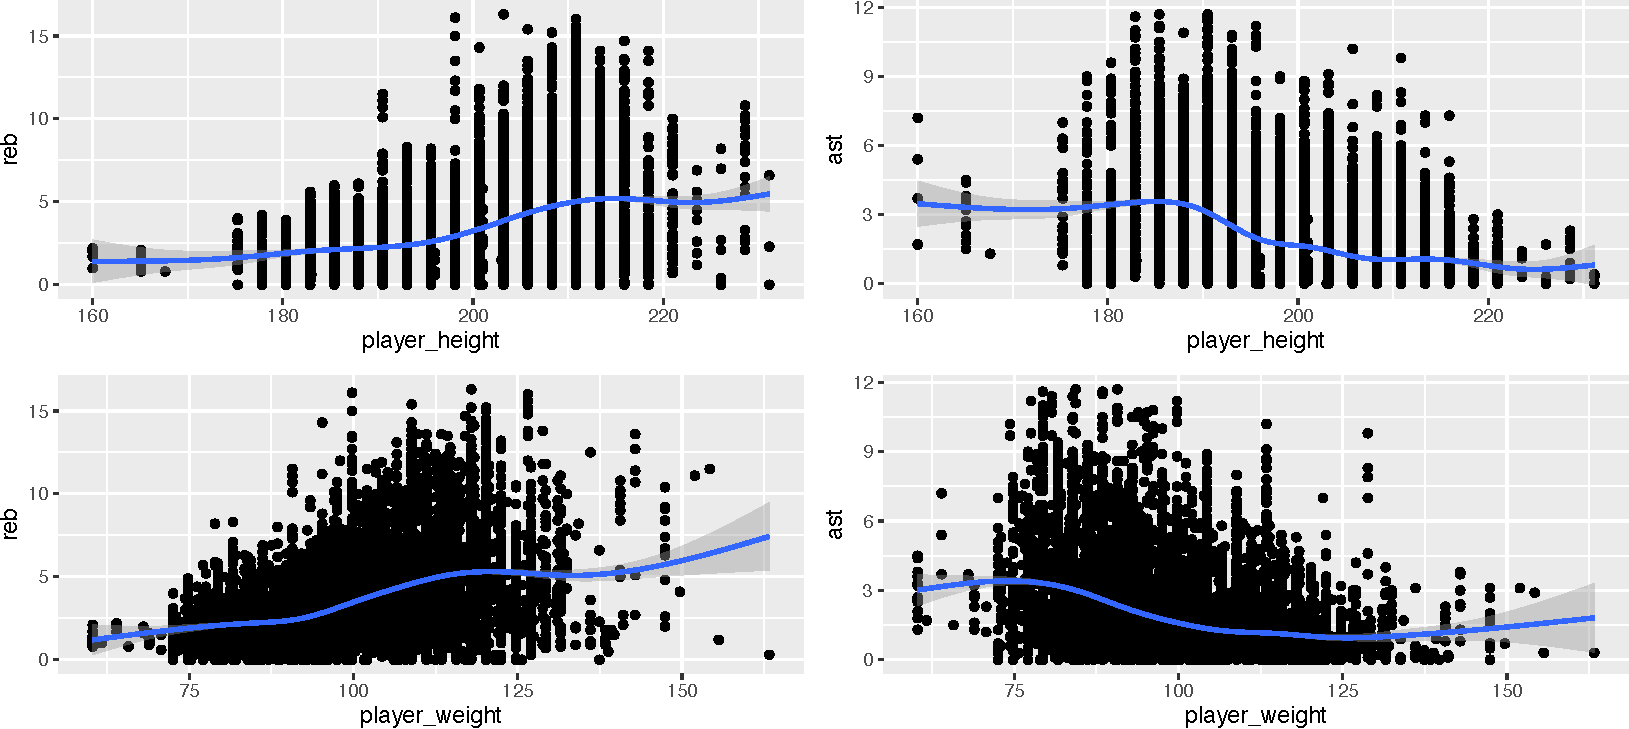
\includegraphics{_main_files/figure-latex/unnamed-chunk-16-1.pdf}

\hypertarget{in-depth-analysis-between-weight-and-height}{%
\chapter{In-depth Analysis Between Weight and Height}\label{in-depth-analysis-between-weight-and-height}}

\begin{Shaded}
\begin{Highlighting}[]
\NormalTok{p1}\OtherTok{\textless{}{-}}\FunctionTok{ggplot}\NormalTok{(nba,}\FunctionTok{aes}\NormalTok{(}\AttributeTok{x=}\NormalTok{player\_weight,}\AttributeTok{y=}\NormalTok{player\_height))}
\NormalTok{p1}\OtherTok{\textless{}{-}}\NormalTok{p1}\SpecialCharTok{+}\FunctionTok{geom\_point}\NormalTok{()}
\NormalTok{p1}\SpecialCharTok{+}\FunctionTok{geom\_smooth}\NormalTok{()}
\end{Highlighting}
\end{Shaded}

\begin{verbatim}
## `geom_smooth()` using method = 'gam' and formula = 'y ~ s(x, bs = "cs")'
\end{verbatim}

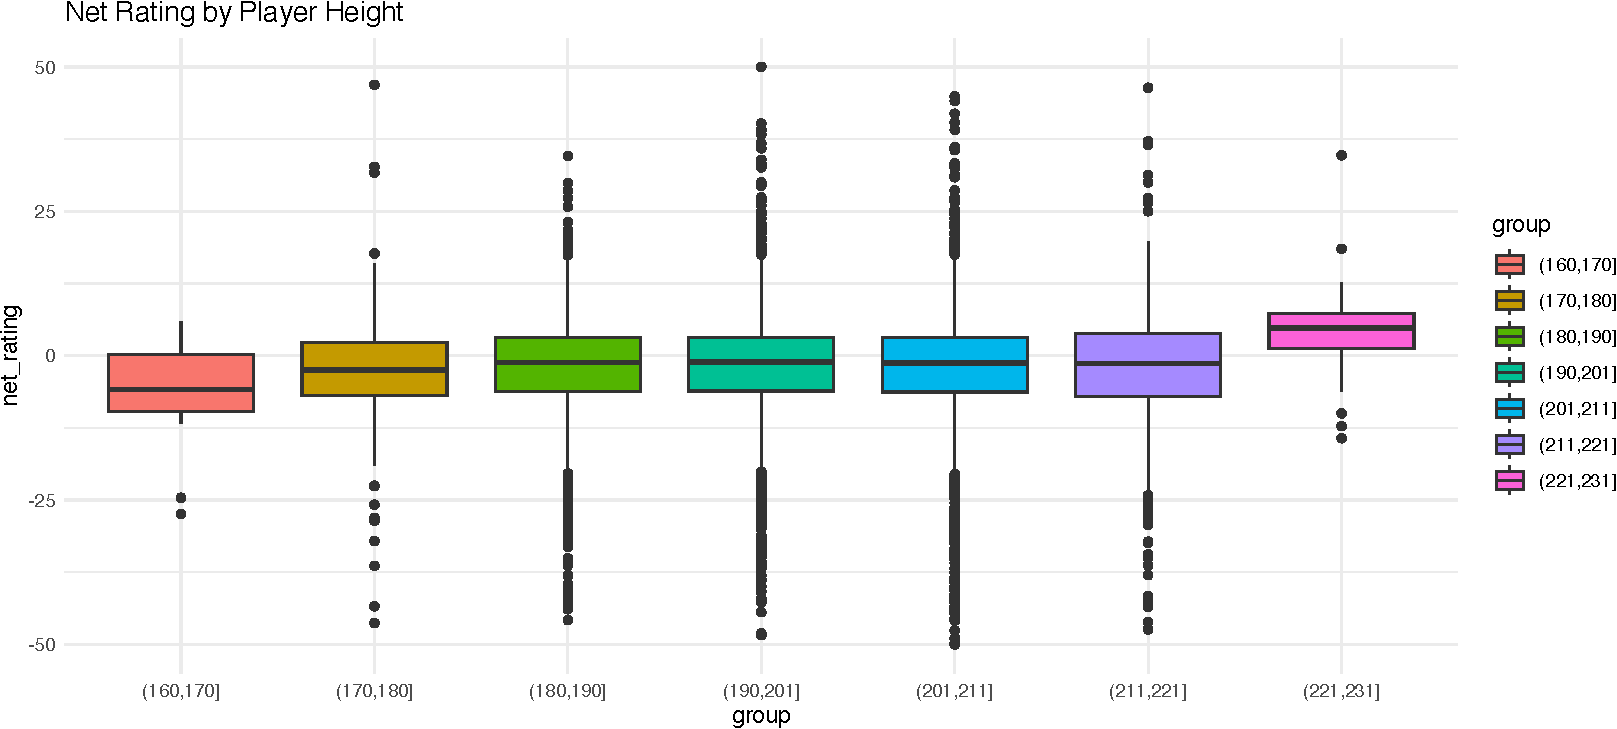
\includegraphics{_main_files/figure-latex/unnamed-chunk-17-1.pdf}

\hypertarget{time-series-visualization}{%
\section{Time-series Visualization}\label{time-series-visualization}}

\begin{Shaded}
\begin{Highlighting}[]
\NormalTok{p }\OtherTok{\textless{}{-}} \FunctionTok{ggplot}\NormalTok{(cor\_df, }\FunctionTok{aes}\NormalTok{(}\AttributeTok{x =}\NormalTok{ season, }\AttributeTok{y =}\NormalTok{ correlation, }\AttributeTok{group =} \DecValTok{1}\NormalTok{)) }\SpecialCharTok{+}  \CommentTok{\# Set group=1 to connect all points}
  \FunctionTok{geom\_line}\NormalTok{() }\SpecialCharTok{+}
  \FunctionTok{xlab}\NormalTok{(}\StringTok{"Season"}\NormalTok{) }\SpecialCharTok{+}
  \FunctionTok{ylab}\NormalTok{(}\StringTok{"Correlation between Height and Weight"}\NormalTok{) }\SpecialCharTok{+}
  \FunctionTok{ggtitle}\NormalTok{(}\StringTok{"Correlation between Height and Weight over Seasons"}\NormalTok{) }\SpecialCharTok{+}
  \FunctionTok{theme\_minimal}\NormalTok{()}
\FunctionTok{print}\NormalTok{(p)}
\end{Highlighting}
\end{Shaded}

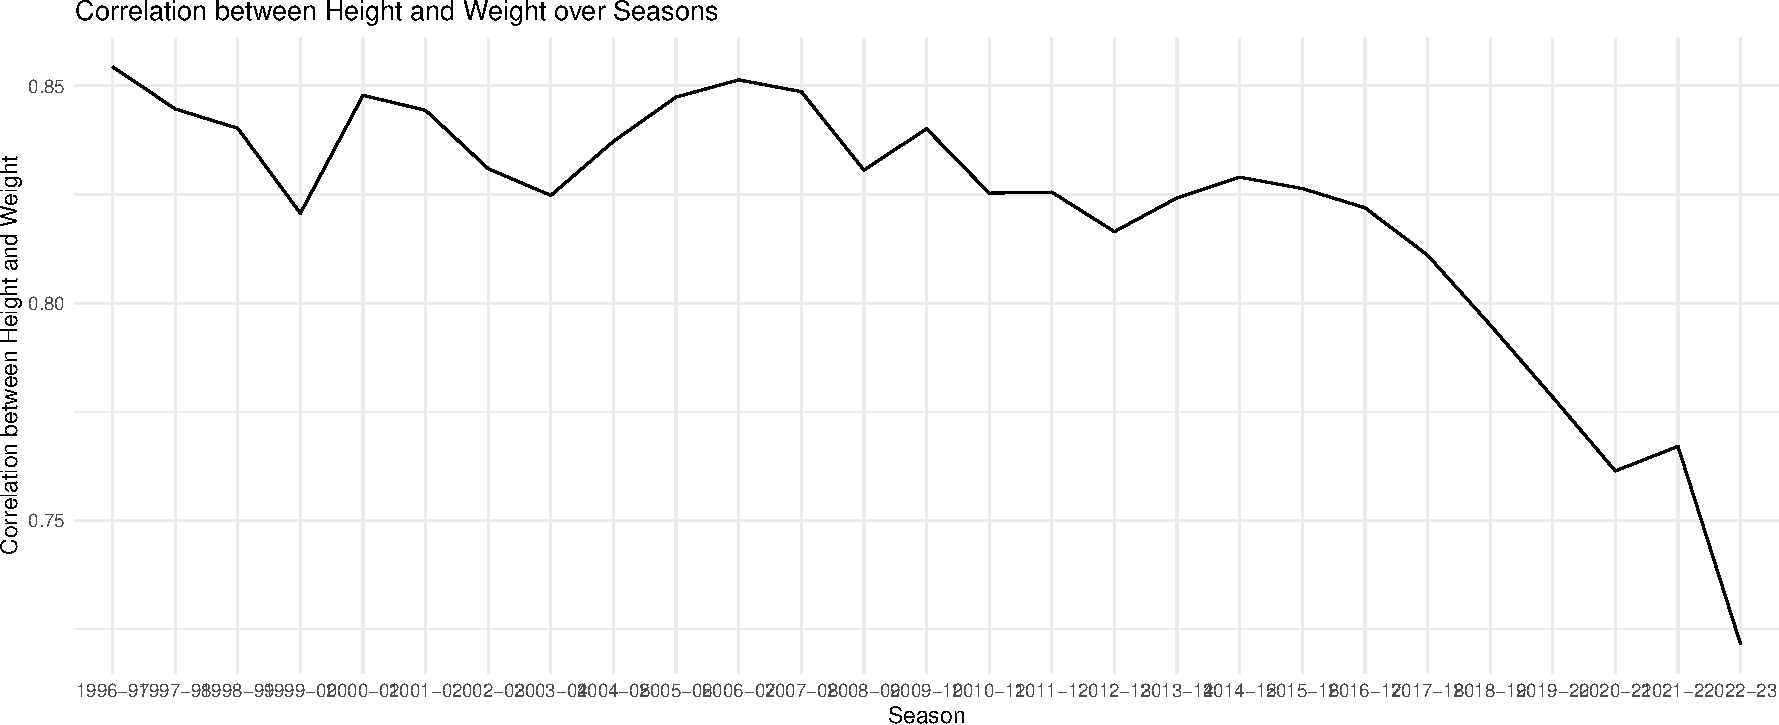
\includegraphics{_main_files/figure-latex/unnamed-chunk-19-1.pdf}

\hypertarget{clustering}{%
\section{Clustering}\label{clustering}}

\hypertarget{k-means-clustering}{%
\subsection{k-means Clustering}\label{k-means-clustering}}

\begin{Shaded}
\begin{Highlighting}[]
\NormalTok{nba\_selected\_season }\OtherTok{\textless{}{-}}\NormalTok{ nba[(}\FunctionTok{which}\NormalTok{(nba}\SpecialCharTok{$}\NormalTok{season }\SpecialCharTok{==} \StringTok{"2022{-}23"}\NormalTok{)),]}
\NormalTok{nba\_selected\_season}\OtherTok{\textless{}{-}}\NormalTok{nba\_selected\_season[nba\_selected\_season}\SpecialCharTok{$}\NormalTok{pts}\SpecialCharTok{\textgreater{}}\DecValTok{10}\NormalTok{,]}
\NormalTok{nba\_selected\_season}\OtherTok{\textless{}{-}}\NormalTok{nba\_selected\_season[nba\_selected\_season}\SpecialCharTok{$}\NormalTok{gp}\SpecialCharTok{\textgreater{}}\DecValTok{50}\NormalTok{,]}
\FunctionTok{rownames}\NormalTok{(nba\_selected\_season)}\OtherTok{\textless{}{-}}\NormalTok{nba\_selected\_season}\SpecialCharTok{$}\NormalTok{player\_name}

\NormalTok{selected\_features }\OtherTok{\textless{}{-}} \FunctionTok{c}\NormalTok{(}\StringTok{\textquotesingle{}player\_height\textquotesingle{}}\NormalTok{, }\StringTok{\textquotesingle{}pts\textquotesingle{}}\NormalTok{,}\StringTok{\textquotesingle{}player\_weight\textquotesingle{}}\NormalTok{, }\StringTok{\textquotesingle{}reb\textquotesingle{}}\NormalTok{, }\StringTok{\textquotesingle{}ast\textquotesingle{}}\NormalTok{, }\StringTok{\textquotesingle{}net\_rating\textquotesingle{}}\NormalTok{,}\StringTok{\textquotesingle{}oreb\_pct\textquotesingle{}}\NormalTok{,}\StringTok{\textquotesingle{}dreb\_pct\textquotesingle{}}\NormalTok{,}\StringTok{\textquotesingle{}usg\_pct\textquotesingle{}}\NormalTok{,}\StringTok{\textquotesingle{}ts\_pct\textquotesingle{}}\NormalTok{,}\StringTok{\textquotesingle{}ast\_pct\textquotesingle{}}\NormalTok{)}
\NormalTok{nba\_for\_clustering }\OtherTok{\textless{}{-}}\NormalTok{ nba\_selected\_season }\SpecialCharTok{\%\textgreater{}\%} \FunctionTok{select}\NormalTok{(}\FunctionTok{all\_of}\NormalTok{(selected\_features))}

\NormalTok{df }\OtherTok{\textless{}{-}} \FunctionTok{as.data.frame}\NormalTok{(}\FunctionTok{scale}\NormalTok{(nba\_for\_clustering))}


\FunctionTok{fviz\_nbclust}\NormalTok{(df, kmeans, }\AttributeTok{method =} \StringTok{"wss"}\NormalTok{) }\SpecialCharTok{+} \FunctionTok{geom\_vline}\NormalTok{(}\AttributeTok{xintercept =} \DecValTok{7}\NormalTok{, }\AttributeTok{linetype =} \DecValTok{2}\NormalTok{) }
\end{Highlighting}
\end{Shaded}

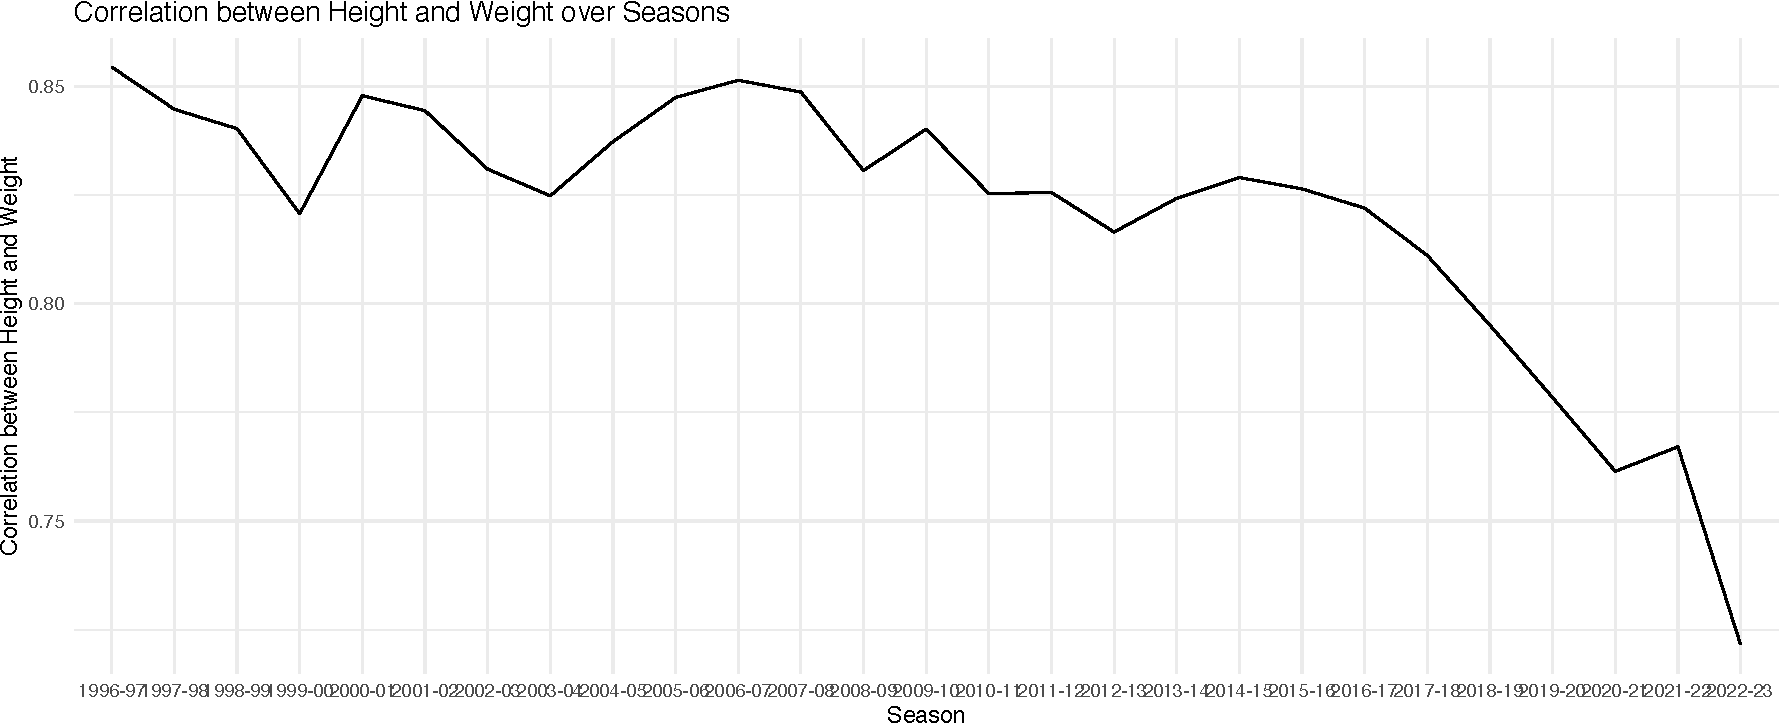
\includegraphics{_main_files/figure-latex/unnamed-chunk-24-1.pdf}

\begin{Shaded}
\begin{Highlighting}[]
\FunctionTok{set.seed}\NormalTok{(}\DecValTok{123}\NormalTok{)}
\NormalTok{km\_result }\OtherTok{\textless{}{-}} \FunctionTok{kmeans}\NormalTok{(df, }\AttributeTok{centers =} \DecValTok{7}\NormalTok{)}
\end{Highlighting}
\end{Shaded}

\begin{Shaded}
\begin{Highlighting}[]
\NormalTok{clustering\_23}\OtherTok{\textless{}{-}}\FunctionTok{fviz\_cluster}\NormalTok{(km\_result, }\AttributeTok{data =}\NormalTok{ df,}
             \AttributeTok{ellipse.type =} \StringTok{"euclid"}\NormalTok{,}
             \AttributeTok{ellipse.level=}\FloatTok{0.5}\NormalTok{,}
             \AttributeTok{ellipse.ratio=}\FloatTok{0.8}\NormalTok{,}
             \AttributeTok{star.plot =} \ConstantTok{TRUE}\NormalTok{,}
             \AttributeTok{repel =} \ConstantTok{TRUE}\NormalTok{,}
             \AttributeTok{main=}\StringTok{"NBA 2022{-}2023"}\NormalTok{,}
             \AttributeTok{ggtheme =} \FunctionTok{theme\_minimal}\NormalTok{())}

\NormalTok{clustering\_23 }\OtherTok{\textless{}{-}}\NormalTok{ clustering\_23 }\SpecialCharTok{+}
  \FunctionTok{theme}\NormalTok{(}
    \AttributeTok{plot.title =} \FunctionTok{element\_text}\NormalTok{(}
      \AttributeTok{size =} \DecValTok{30}\NormalTok{,               }
      \AttributeTok{face =} \StringTok{"italic"}\NormalTok{,}
      \AttributeTok{color =} \StringTok{"blue"}\NormalTok{,          }
      \AttributeTok{hjust =} \FloatTok{0.5}\NormalTok{,            }
      \AttributeTok{vjust =} \DecValTok{1}\NormalTok{,               }
      \AttributeTok{angle =} \DecValTok{0}\NormalTok{,               }
      \AttributeTok{lineheight =} \FloatTok{1.2}         
\NormalTok{    )}
\NormalTok{  )}
\end{Highlighting}
\end{Shaded}

For season 1999-00

\begin{Shaded}
\begin{Highlighting}[]
\FunctionTok{print}\NormalTok{(clustering\_00)}
\end{Highlighting}
\end{Shaded}

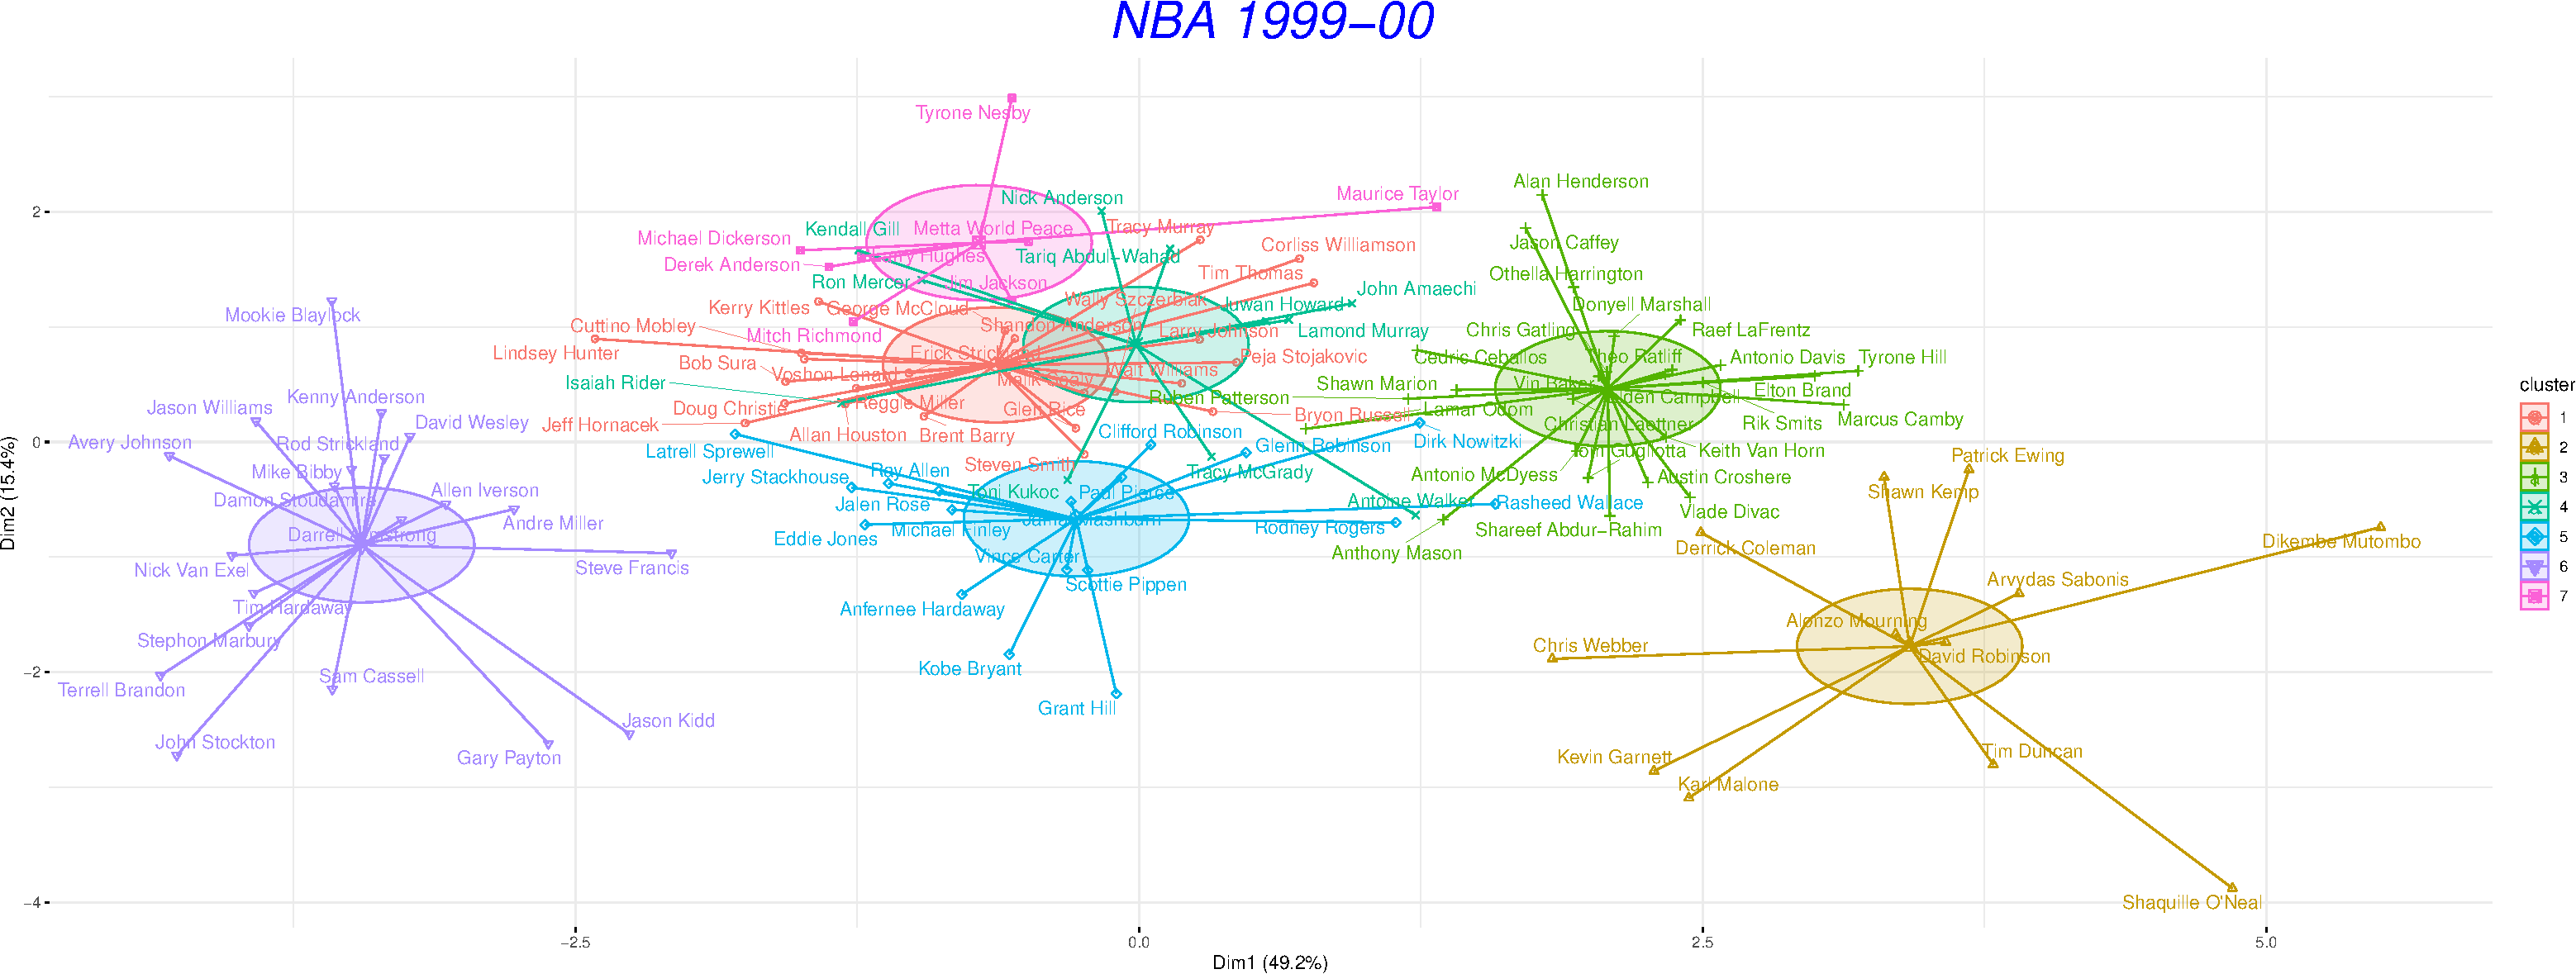
\includegraphics{_main_files/figure-latex/unnamed-chunk-27-1.pdf}

\begin{Shaded}
\begin{Highlighting}[]
\FunctionTok{kable}\NormalTok{(mean\_values\_00)}
\end{Highlighting}
\end{Shaded}

\begin{tabular}{r|r|r|r|r|r}
\hline
cluster & player\_height & player\_weight & pts & reb & ast\\
\hline
1 & 198.9667 & 96.38830 & 12.92917 & 3.879167 & 2.558333\\
\hline
2 & 212.3017 & 119.63489 & 19.84167 & 10.483333 & 2.650000\\
\hline
3 & 207.4008 & 108.30381 & 13.78462 & 7.665385 & 1.826923\\
\hline
4 & 202.0455 & 104.65605 & 14.86364 & 5.009091 & 2.709091\\
\hline
5 & 201.9300 & 99.89104 & 19.59444 & 5.505556 & 3.811111\\
\hline
6 & 186.1820 & 83.95988 & 15.68500 & 3.680000 & 7.250000\\
\hline
7 & 197.8025 & 98.59956 & 15.82500 & 4.275000 & 2.475000\\
\hline
\end{tabular}

For season 2009-10

\begin{Shaded}
\begin{Highlighting}[]
\FunctionTok{print}\NormalTok{(clustering\_10)}
\end{Highlighting}
\end{Shaded}

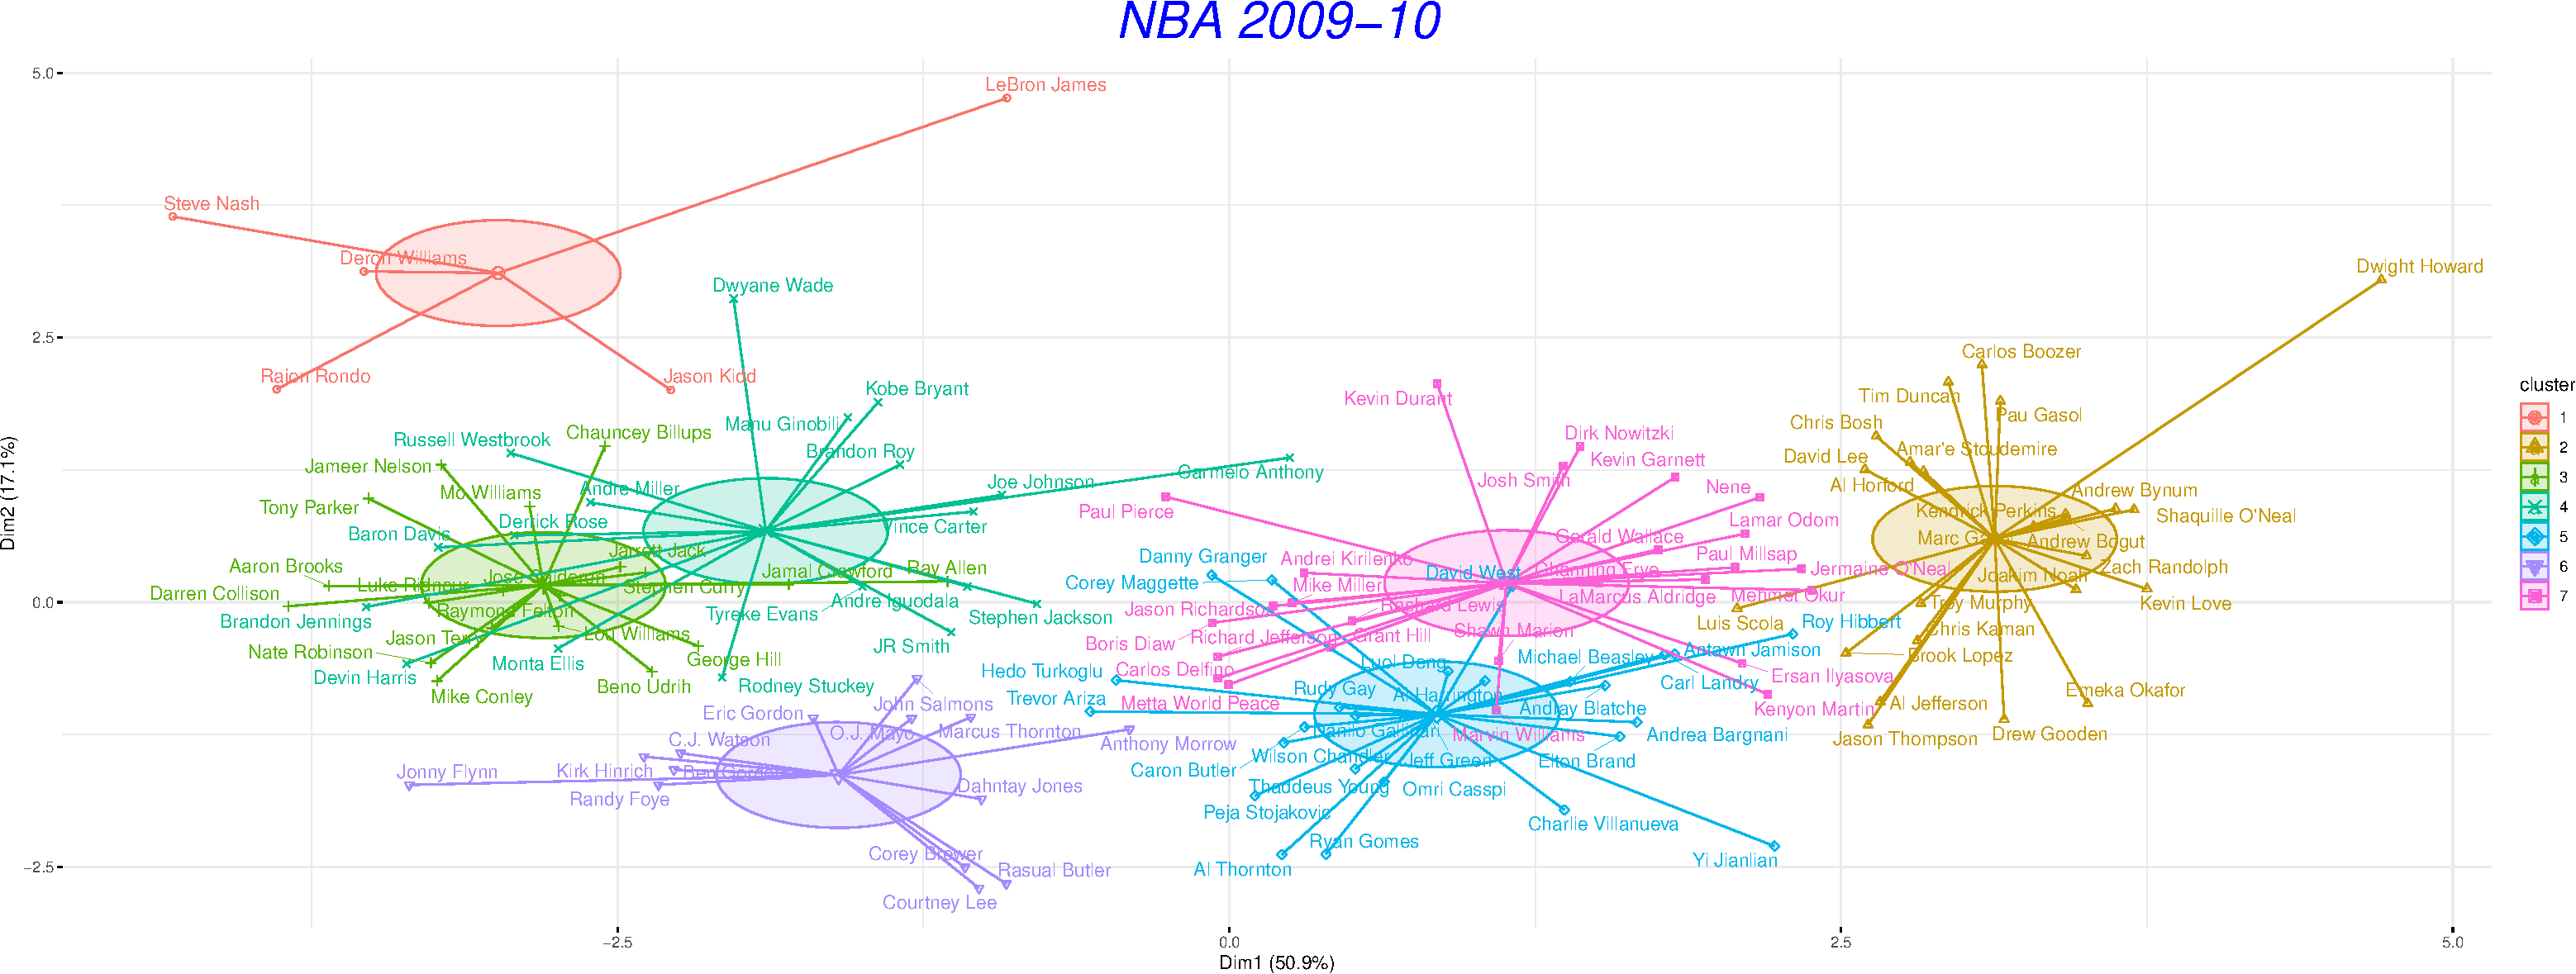
\includegraphics{_main_files/figure-latex/unnamed-chunk-30-1.pdf}

\begin{Shaded}
\begin{Highlighting}[]
\FunctionTok{kable}\NormalTok{(mean\_values\_10)}
\end{Highlighting}
\end{Shaded}

\begin{tabular}{r|r|r|r|r|r}
\hline
cluster & player\_height & player\_weight & pts & reb & ast\\
\hline
1 & 192.5320 & 92.16989 & 17.78000 & 4.920000 & 9.800000\\
\hline
2 & 210.0792 & 117.59373 & 16.15000 & 9.754167 & 1.991667\\
\hline
3 & 187.4253 & 84.94107 & 14.20526 & 2.705263 & 4.673684\\
\hline
4 & 195.1789 & 93.79805 & 19.55789 & 4.378947 & 5.252632\\
\hline
5 & 206.3262 & 106.50689 & 15.16923 & 5.715385 & 1.834615\\
\hline
6 & 193.9471 & 91.36639 & 13.10714 & 2.964286 & 2.650000\\
\hline
7 & 205.5446 & 107.67576 & 14.13462 & 6.519231 & 2.338462\\
\hline
\end{tabular}

For season 2015-16

\begin{Shaded}
\begin{Highlighting}[]
\FunctionTok{print}\NormalTok{(clustering\_16)}
\end{Highlighting}
\end{Shaded}

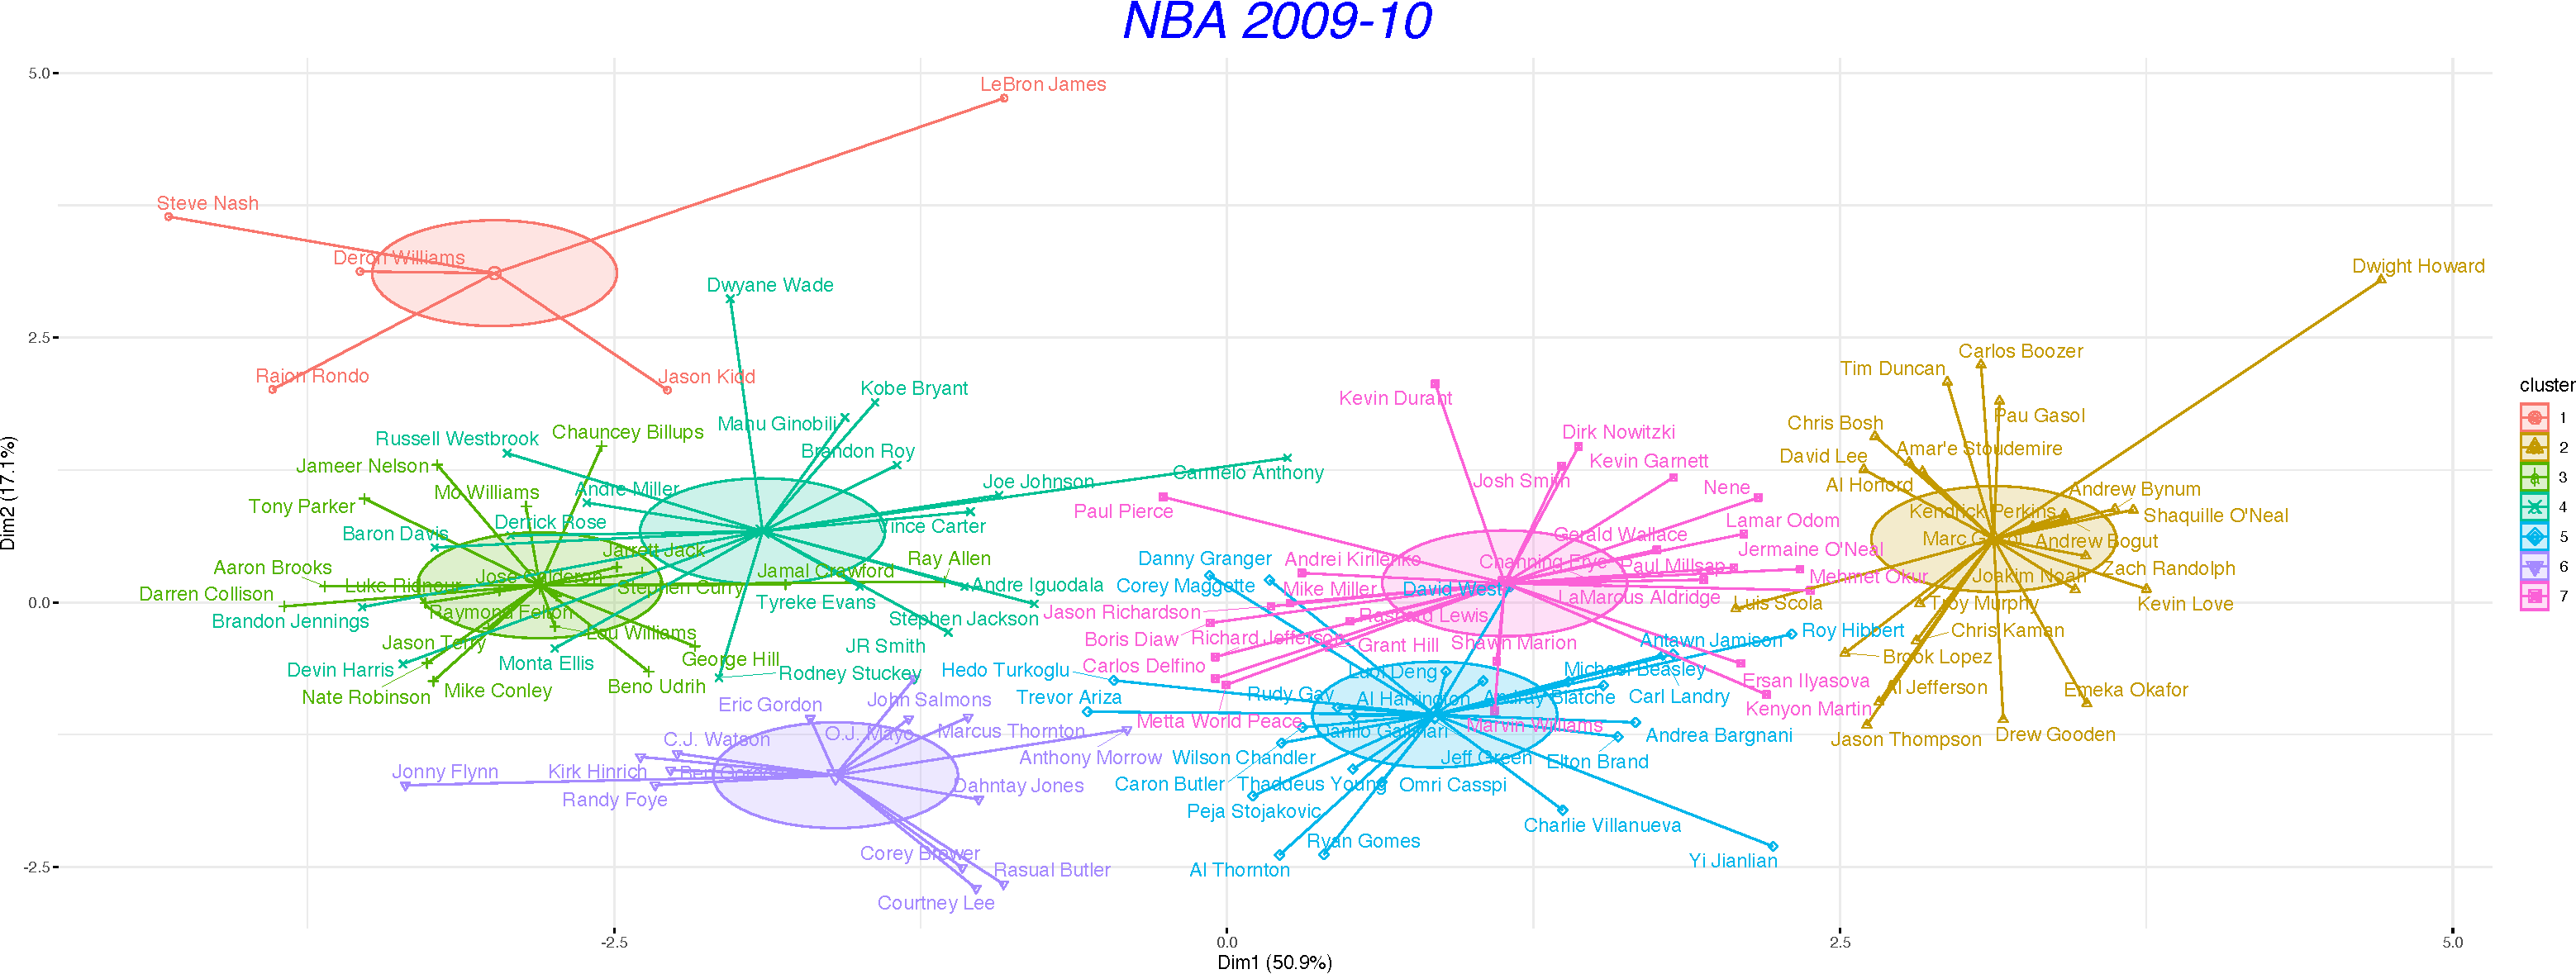
\includegraphics{_main_files/figure-latex/unnamed-chunk-33-1.pdf}

\begin{Shaded}
\begin{Highlighting}[]
\FunctionTok{kable}\NormalTok{(mean\_values\_16)}
\end{Highlighting}
\end{Shaded}

\begin{tabular}{r|r|r|r|r|r}
\hline
cluster & player\_height & player\_weight & pts & reb & ast\\
\hline
1 & 189.7592 & 88.50714 & 17.87917 & 4.016667 & 6.491667\\
\hline
2 & 209.5500 & 114.50930 & 16.73000 & 8.585000 & 2.370000\\
\hline
3 & 191.5459 & 87.30312 & 13.50000 & 3.147059 & 3.817647\\
\hline
4 & 196.7593 & 94.16894 & 14.13929 & 3.557143 & 2.671429\\
\hline
5 & 211.0509 & 114.71754 & 13.36364 & 10.263636 & 1.145455\\
\hline
6 & 206.3262 & 104.76231 & 13.67692 & 5.723077 & 1.788461\\
\hline
7 & 201.0229 & 102.05820 & 23.42857 & 6.871429 & 4.957143\\
\hline
\end{tabular}

For season 2022-23

\begin{Shaded}
\begin{Highlighting}[]
\FunctionTok{print}\NormalTok{(clustering\_23)}
\end{Highlighting}
\end{Shaded}

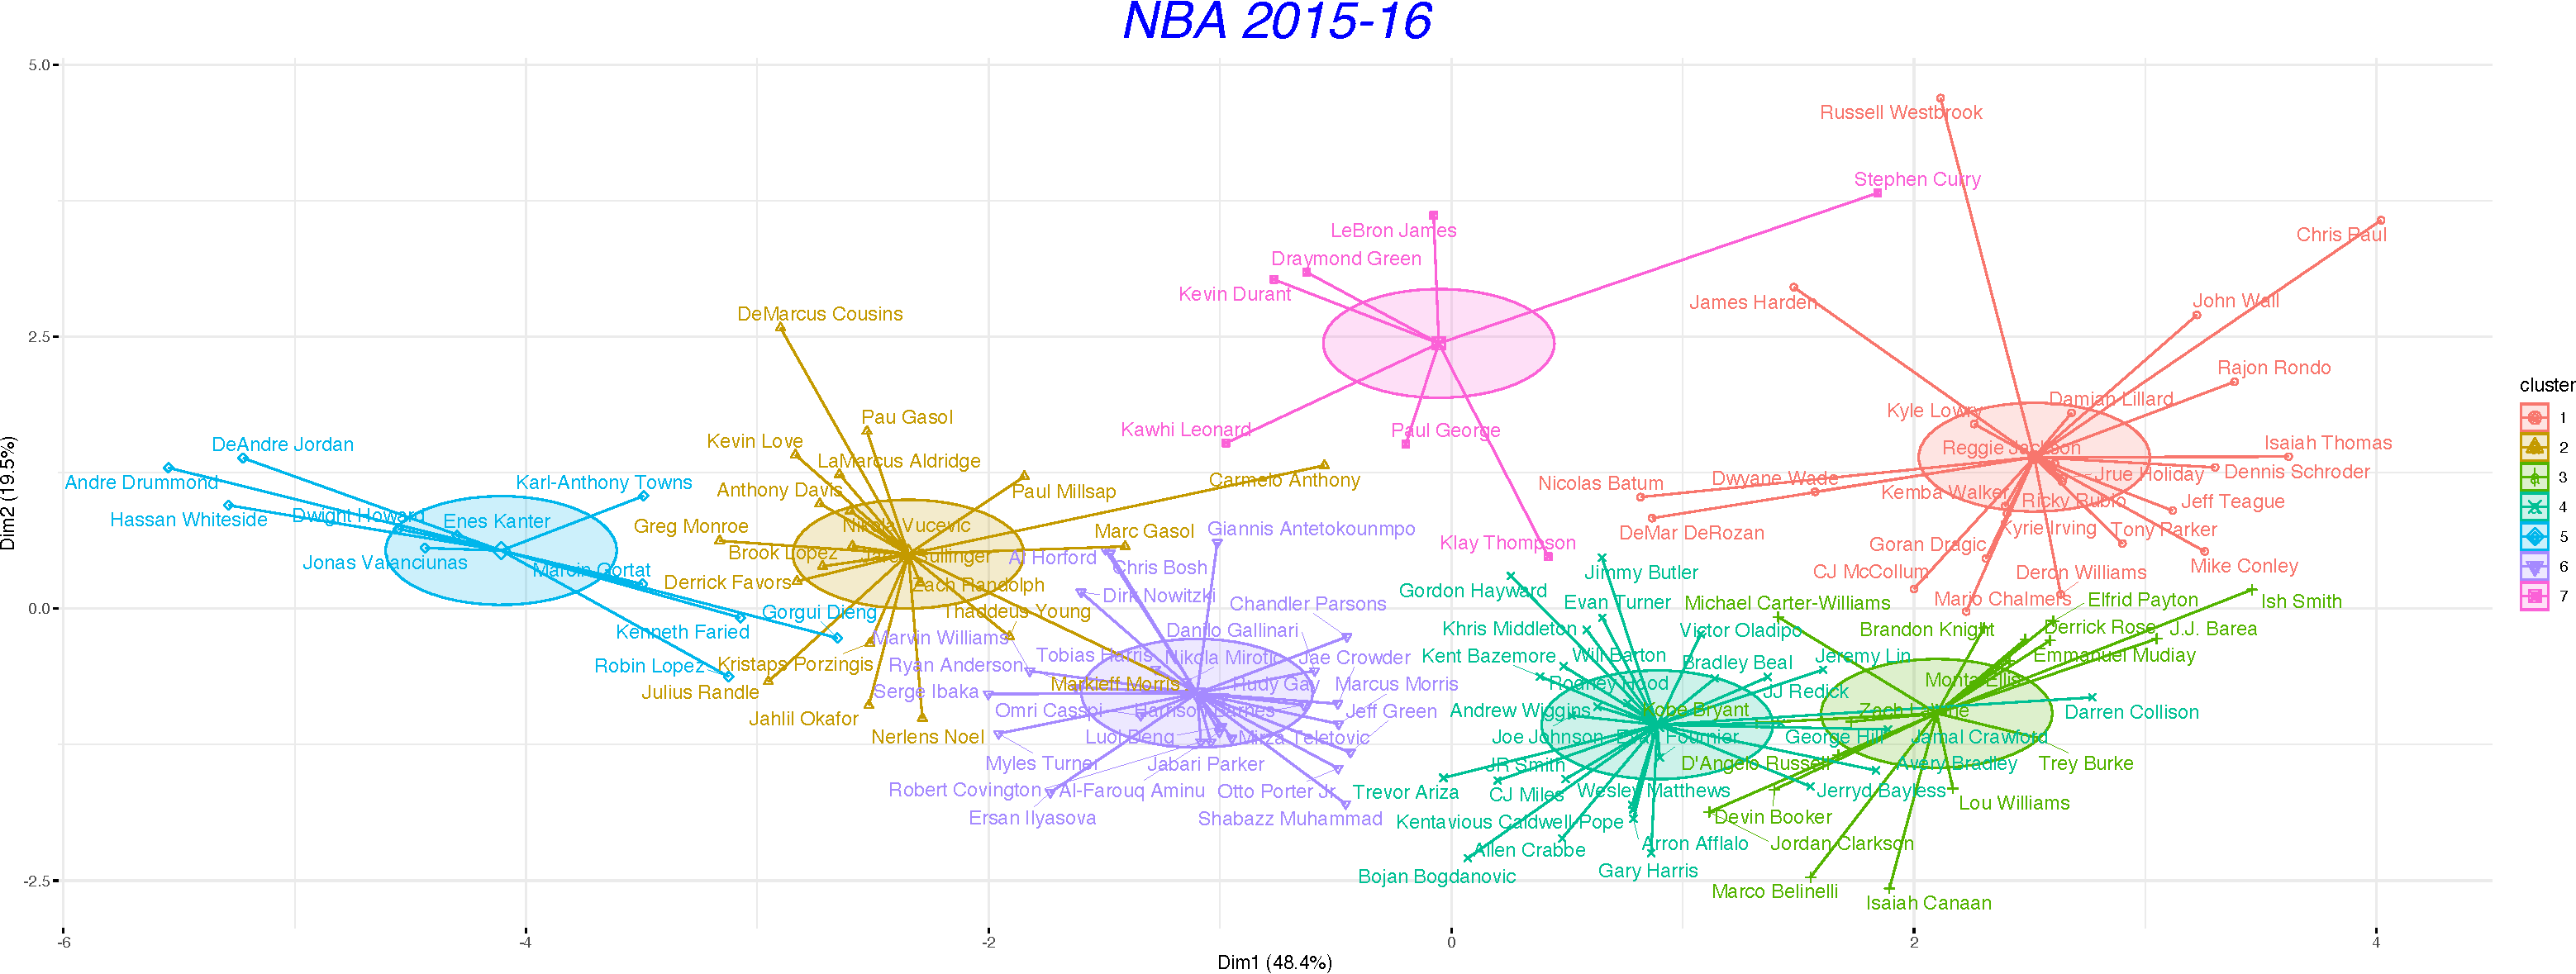
\includegraphics{_main_files/figure-latex/unnamed-chunk-36-1.pdf}

\begin{Shaded}
\begin{Highlighting}[]
\FunctionTok{kable}\NormalTok{(mean\_values\_23)}
\end{Highlighting}
\end{Shaded}

\begin{tabular}{r|r|r|r|r|r}
\hline
cluster & player\_height & player\_weight & pts & reb & ast\\
\hline
1 & 211.3280 & 113.25285 & 15.90000 & 9.196000 & 2.352000\\
\hline
2 & 197.4615 & 97.10229 & 13.09259 & 3.555556 & 1.855556\\
\hline
3 & 206.6925 & 112.09392 & 28.67500 & 9.662500 & 6.125000\\
\hline
4 & 189.2300 & 88.18241 & 13.73182 & 3.427273 & 5.009091\\
\hline
5 & 201.2462 & 98.91795 & 14.81154 & 4.538462 & 2.276923\\
\hline
6 & 193.2609 & 92.27639 & 24.90000 & 4.917391 & 6.239130\\
\hline
7 & 195.5800 & 92.41340 & 18.14737 & 4.826316 & 4.700000\\
\hline
\end{tabular}

\hypertarget{hierachical-clustering}{%
\subsection{Hierachical Clustering}\label{hierachical-clustering}}

\begin{Shaded}
\begin{Highlighting}[]
\NormalTok{result\_23 }\OtherTok{\textless{}{-}} \FunctionTok{dist}\NormalTok{(df, }\AttributeTok{method =} \StringTok{"euclidean"}\NormalTok{)}
\NormalTok{result\_hc }\OtherTok{\textless{}{-}} \FunctionTok{hclust}\NormalTok{(}\AttributeTok{d =}\NormalTok{ result\_23, }\AttributeTok{method =} \StringTok{"ward.D2"}\NormalTok{)}
\FunctionTok{fviz\_dend}\NormalTok{(result\_hc, }\AttributeTok{k =} \DecValTok{4}\NormalTok{,}
          \AttributeTok{cex =} \FloatTok{0.5}\NormalTok{,}
          \AttributeTok{color\_labels\_by\_k =} \ConstantTok{TRUE}\NormalTok{,}
          \AttributeTok{main=}\StringTok{"NBA 2022{-}2023"}\NormalTok{,}
          \AttributeTok{rect =} \ConstantTok{TRUE}
\NormalTok{)}
\end{Highlighting}
\end{Shaded}

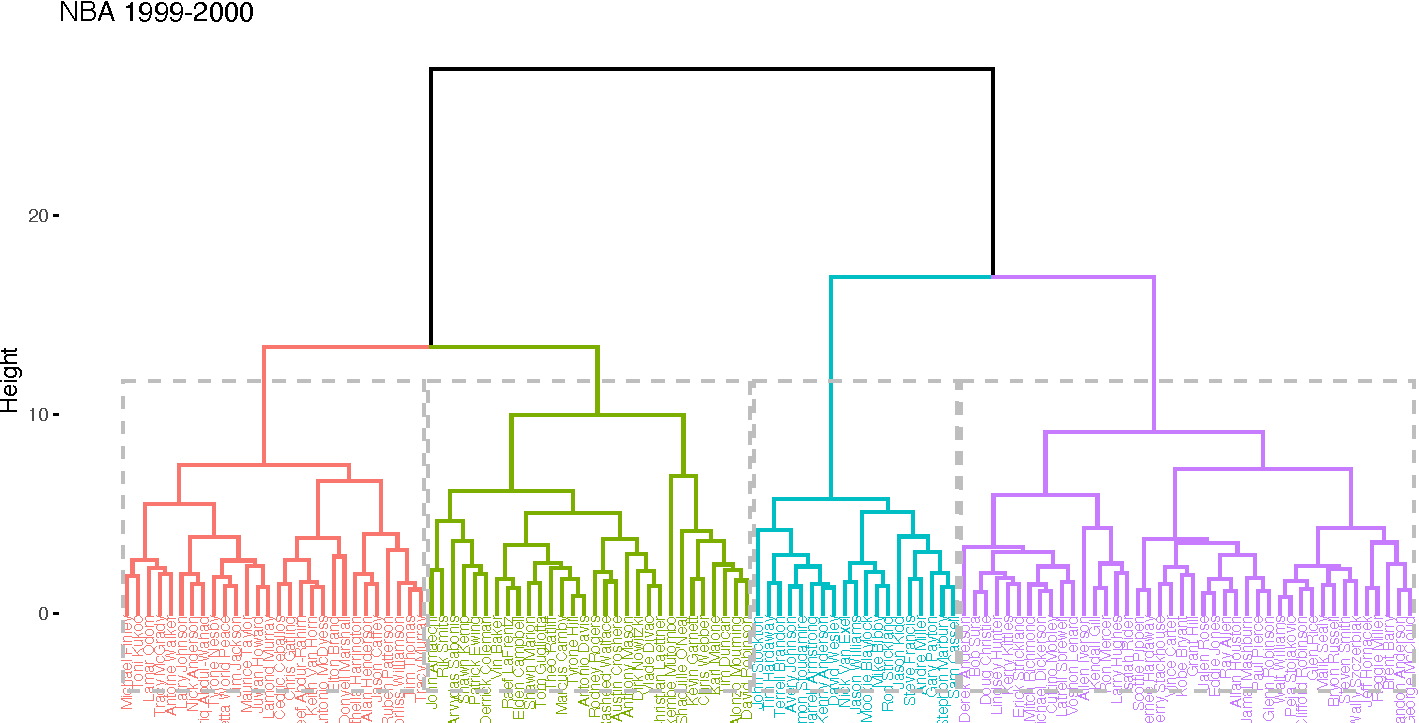
\includegraphics{_main_files/figure-latex/unnamed-chunk-40-1.pdf}

\begin{Shaded}
\begin{Highlighting}[]
\FunctionTok{fviz\_dend}\NormalTok{(result\_hc\_00, }\AttributeTok{k =} \DecValTok{4}\NormalTok{,}
          \AttributeTok{cex =} \FloatTok{0.5}\NormalTok{,}
          \AttributeTok{color\_labels\_by\_k =} \ConstantTok{TRUE}\NormalTok{,}
          \AttributeTok{main=}\StringTok{"NBA 1999{-}2000"}\NormalTok{,}
          \AttributeTok{rect =} \ConstantTok{TRUE}
\NormalTok{)}
\end{Highlighting}
\end{Shaded}

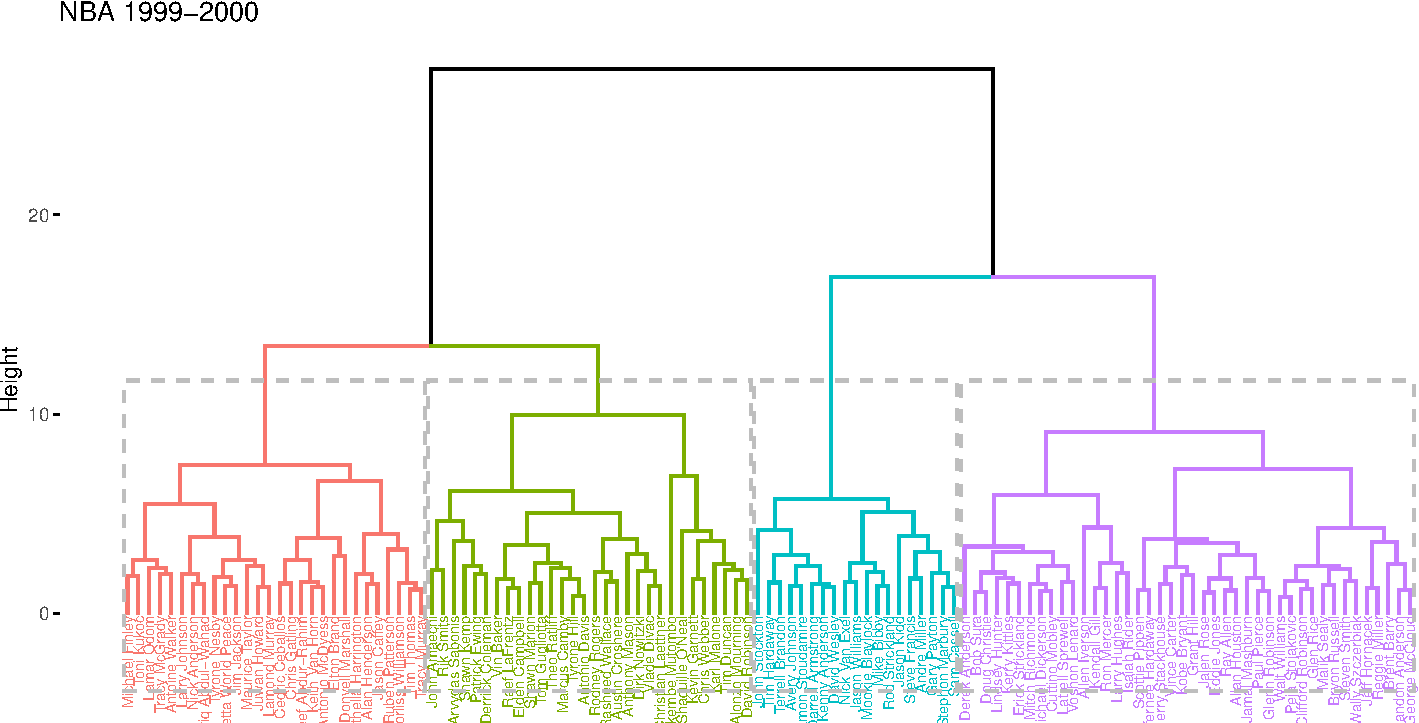
\includegraphics{_main_files/figure-latex/unnamed-chunk-41-1.pdf}

\begin{Shaded}
\begin{Highlighting}[]
\FunctionTok{fviz\_dend}\NormalTok{(result\_hc\_10, }\AttributeTok{k =} \DecValTok{4}\NormalTok{,}
          \AttributeTok{cex =} \FloatTok{0.5}\NormalTok{,}
          \AttributeTok{color\_labels\_by\_k =} \ConstantTok{TRUE}\NormalTok{,}
          \AttributeTok{main=}\StringTok{"NBA 2009{-}2010"}\NormalTok{,}
          \AttributeTok{rect =} \ConstantTok{TRUE}
\NormalTok{)}
\end{Highlighting}
\end{Shaded}

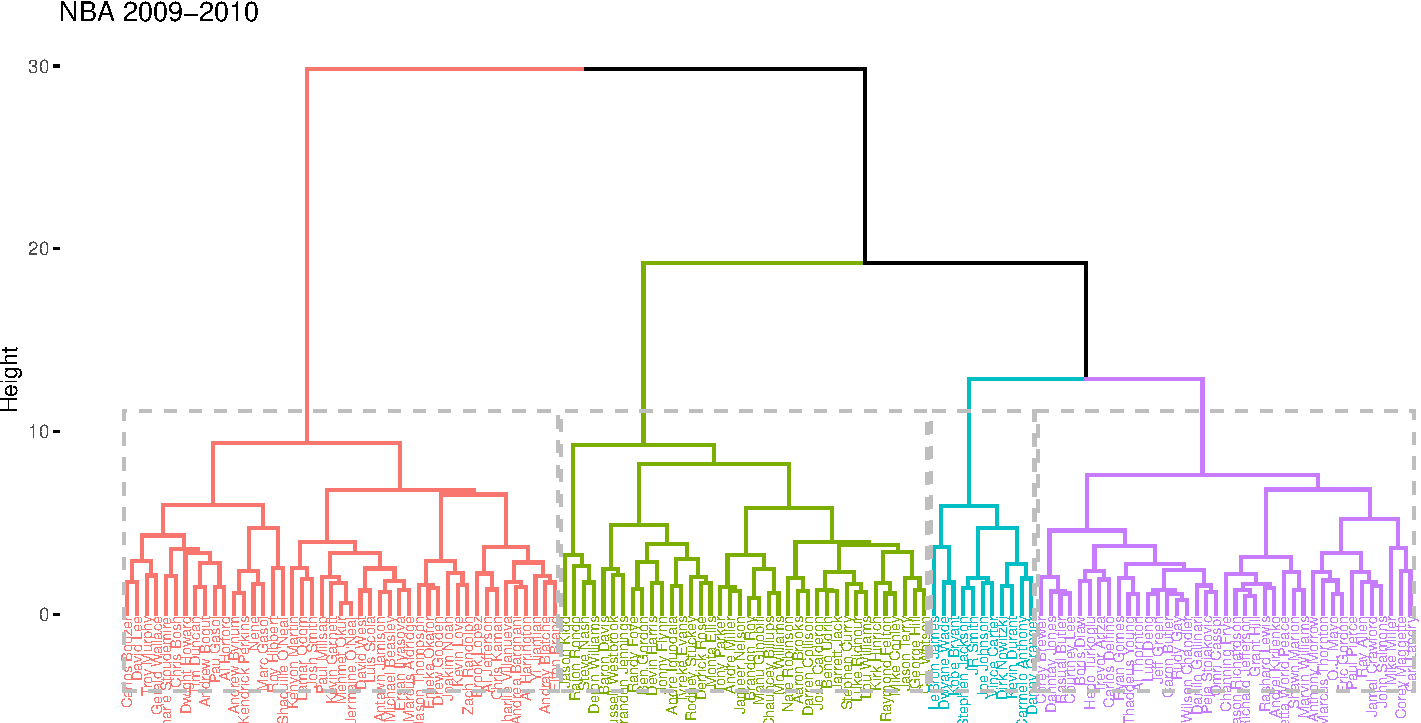
\includegraphics{_main_files/figure-latex/unnamed-chunk-41-2.pdf}

\begin{Shaded}
\begin{Highlighting}[]
\FunctionTok{fviz\_dend}\NormalTok{(result\_hc\_16, }\AttributeTok{k =} \DecValTok{4}\NormalTok{,}
          \AttributeTok{cex =} \FloatTok{0.5}\NormalTok{,}
          \AttributeTok{color\_labels\_by\_k =} \ConstantTok{TRUE}\NormalTok{,}
          \AttributeTok{main=}\StringTok{"NBA 2015{-}2016"}\NormalTok{,}
          \AttributeTok{rect =} \ConstantTok{TRUE}
\NormalTok{)}
\end{Highlighting}
\end{Shaded}

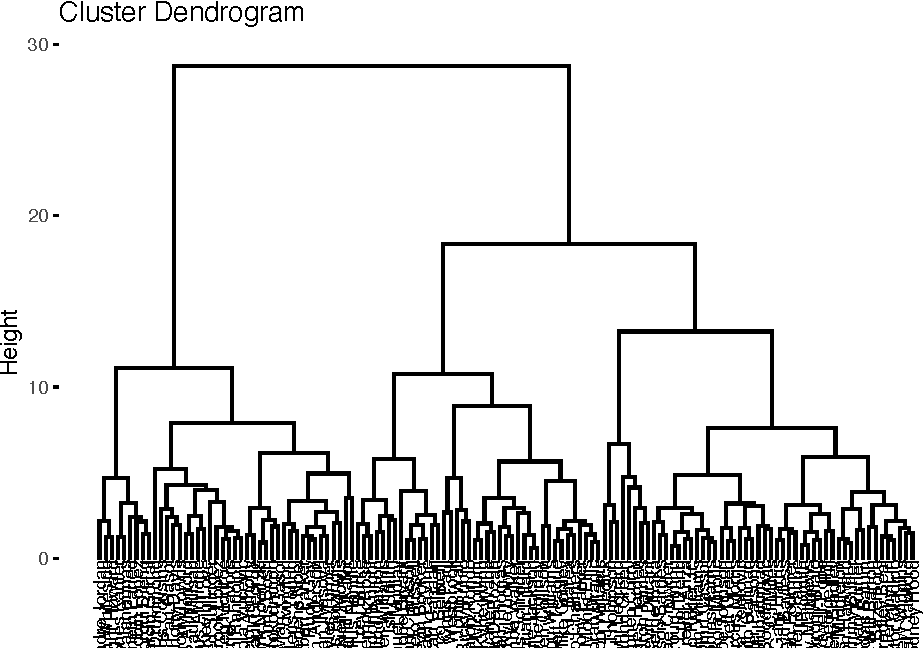
\includegraphics{_main_files/figure-latex/unnamed-chunk-41-3.pdf}

\hypertarget{parts}{%
\chapter{Parts}\label{parts}}

You can add parts to organize one or more book chapters together. Parts can be inserted at the top of an .Rmd file, before the first-level chapter heading in that same file.

Add a numbered part: \texttt{\#\ (PART)\ Act\ one\ \{-\}} (followed by \texttt{\#\ A\ chapter})

Add an unnumbered part: \texttt{\#\ (PART\textbackslash{}*)\ Act\ one\ \{-\}} (followed by \texttt{\#\ A\ chapter})

Add an appendix as a special kind of un-numbered part: \texttt{\#\ (APPENDIX)\ Other\ stuff\ \{-\}} (followed by \texttt{\#\ A\ chapter}). Chapters in an appendix are prepended with letters instead of numbers.

\hypertarget{footnotes-and-citations}{%
\chapter{Footnotes and citations}\label{footnotes-and-citations}}

\hypertarget{footnotes}{%
\section{Footnotes}\label{footnotes}}

Footnotes are put inside the square brackets after a caret \texttt{\^{}{[}{]}}. Like this one \footnote{This is a footnote.}.

\hypertarget{citations}{%
\section{Citations}\label{citations}}

Reference items in your bibliography file(s) using \texttt{@key}.

For example, we are using the \textbf{bookdown} package \citep{R-bookdown} (check out the last code chunk in index.Rmd to see how this citation key was added) in this sample book, which was built on top of R Markdown and \textbf{knitr} \citep{xie2015} (this citation was added manually in an external file book.bib).
Note that the \texttt{.bib} files need to be listed in the index.Rmd with the YAML \texttt{bibliography} key.

The RStudio Visual Markdown Editor can also make it easier to insert citations: \url{https://rstudio.github.io/visual-markdown-editing/\#/citations}

\hypertarget{blocks}{%
\chapter{Blocks}\label{blocks}}

\hypertarget{equations}{%
\section{Equations}\label{equations}}

Here is an equation.

\begin{equation} 
  f\left(k\right) = \binom{n}{k} p^k\left(1-p\right)^{n-k}
  \label{eq:binom}
\end{equation}

You may refer to using \texttt{\textbackslash{}@ref(eq:binom)}, like see Equation \eqref{eq:binom}.

\hypertarget{theorems-and-proofs}{%
\section{Theorems and proofs}\label{theorems-and-proofs}}

Labeled theorems can be referenced in text using \texttt{\textbackslash{}@ref(thm:tri)}, for example, check out this smart theorem \ref{thm:tri}.

\begin{theorem}
\protect\hypertarget{thm:tri}{}\label{thm:tri}For a right triangle, if \(c\) denotes the \emph{length} of the hypotenuse
and \(a\) and \(b\) denote the lengths of the \textbf{other} two sides, we have
\[a^2 + b^2 = c^2\]
\end{theorem}

Read more here \url{https://bookdown.org/yihui/bookdown/markdown-extensions-by-bookdown.html}.

\hypertarget{callout-blocks}{%
\section{Callout blocks}\label{callout-blocks}}

The R Markdown Cookbook provides more help on how to use custom blocks to design your own callouts: \url{https://bookdown.org/yihui/rmarkdown-cookbook/custom-blocks.html}

\hypertarget{sharing-your-book}{%
\chapter{Sharing your book}\label{sharing-your-book}}

\hypertarget{publishing}{%
\section{Publishing}\label{publishing}}

HTML books can be published online, see: \url{https://bookdown.org/yihui/bookdown/publishing.html}

\hypertarget{pages}{%
\section{404 pages}\label{pages}}

By default, users will be directed to a 404 page if they try to access a webpage that cannot be found. If you'd like to customize your 404 page instead of using the default, you may add either a \texttt{\_404.Rmd} or \texttt{\_404.md} file to your project root and use code and/or Markdown syntax.

\hypertarget{metadata-for-sharing}{%
\section{Metadata for sharing}\label{metadata-for-sharing}}

Bookdown HTML books will provide HTML metadata for social sharing on platforms like Twitter, Facebook, and LinkedIn, using information you provide in the \texttt{index.Rmd} YAML. To setup, set the \texttt{url} for your book and the path to your \texttt{cover-image} file. Your book's \texttt{title} and \texttt{description} are also used.

This \texttt{gitbook} uses the same social sharing data across all chapters in your book- all links shared will look the same.

Specify your book's source repository on GitHub using the \texttt{edit} key under the configuration options in the \texttt{\_output.yml} file, which allows users to suggest an edit by linking to a chapter's source file.

Read more about the features of this output format here:

\url{https://pkgs.rstudio.com/bookdown/reference/gitbook.html}

Or use:

\begin{Shaded}
\begin{Highlighting}[]
\NormalTok{?bookdown}\SpecialCharTok{::}\NormalTok{gitbook}
\end{Highlighting}
\end{Shaded}


  \bibliography{book.bib,packages.bib}

\end{document}
